\chapter{附录}\label{chap:appendix}

\section{基于机器学习对南加州地区的地震中期预报}\label{sec:appendix_seismic}

\subsection{表和图}\label{sec:seis_table_figure}

{\footnotesize
\begin{longtable}{cclcccccccc}
  \bicaption[不同模型预测区块2至区块6未来1年最大震级的拟合指标效果(数据集划分比例为0.8:0.2)]{不同模型预测区块2至区块6未来1年最大震级的拟合指标效果(数据集划分比例为0.8:0.2)。}{The metrics for predicting the maximum magnitute from block 2 to block 6 with the split ratio 0.8:0.2 in next year by different models.}
  \label{tab:seism_block} \\
  \toprule
  \multirow{2}*{区块序号} & \multirow{2}*{模型} & \multicolumn{2}{c}{训练集} & \multicolumn{2}{c}{验证集} \\
  \cmidrule(lr){3-4} \cmidrule(lr){5-6} \noalign{\smallskip}
  & & MSE & RMSE & MSE & RMSE \\
  \midrule
  \endfirsthead 

  \bicaption[不同模型预测区块2至区块6未来1年最大震级的拟合指标效果(数据集划分比例为0.8:0.2)]{不同模型预测区块2至区块6未来1年最大震级的拟合指标效果(数据集划分比例为0.8:0.2)。}{The metrics for predicting the maximum magnitute from block 2 to block 6 with the split ratio 0.8:0.2 in next year by different models (continued).} \\
  \toprule
  \multirow{2}*{区块序号} & \multirow{2}*{模型} & \multicolumn{2}{c}{训练集} & \multicolumn{2}{c}{测试集} \\
  \cmidrule(lr){3-4} \cmidrule(lr){5-6} \noalign{\smallskip}
  & & MSE & RMSE & MSE & RMSE \\
  \midrule
  \endhead 

  \bottomrule
  \endfoot

  2 & LSTM & 0.0129 & 0.1138 & 0.0290 & 0.1703  \\
   & SVR & 0.0162 & 0.1274 & 0.0511 & 0.2261 \\
   & LR & 0.0118 & 0.1085 & 0.2937 & 0.5419\\
   & RF & 0.0045 & 0.0668 & 0.0654 & 0.2557 \\
   & GBRT & 0.0023 & 0.0478 & 0.0666 & 0.2580 \\
   & DT & \textbf{0.0000} & \textbf{0.0000} & 0.2584 & 0.5083 \\
   & KNN & \textbf{0.0000} & \textbf{0.0000} & 0.0525 & 0.2290 \\
   & ETR & \textbf{0.0000} & \textbf{0.0000} & 0.0602 & 0.2453 \\
  \hline
  3 & LSTM & 0.0085 & 0.0920 & 0.2715 & 0.5210  \\
   & SVR & 0.0104 & 0.1019 & 0.5286 & 0.7271 \\
   & LR & 0.0072 & 0.0848 & 0.3738 & 0.6114 \\
   & RF & 0.0019 & 0.0438 & 0.0546 & 0.2337 \\
   & GBRT & 0.0017 & 0.0412 & 0.0399 & 0.1999 \\
   & DT & \textbf{0.0000} & \textbf{0.0000} & 0.0787 & 0.2805 \\
   & KNN & \textbf{0.0000} & \textbf{0.0000} & 0.0843 & 0.2903 \\
   & ETR & \textbf{0.0000} & \textbf{0.0000} & 0.0621 & 0.2491 \\
  \hline
  4 & LSTM & 0.0101 & 0.1006 & 0.0263 & 0.1623 \\
   & SVR & 0.0131 & 0.1143 & 0.0397 & 0.1991  \\
   & LR & 0.0075 & 0.0863 & 0.2995 & 0.5473  \\
   & RF & 0.0020 & 0.0447 & 0.0478 & 0.2187  \\
   & GBRT & 0.0018 & 0.0420 & 0.0188 & 0.1371  \\
   & DT & \textbf{0.0000} & \textbf{0.0000} & 0.0344 & 0.1856 \\
   & KNN & \textbf{0.0000} & \textbf{0.0000} & 0.0226 & 0.1502 \\
   & ETR & \textbf{0.0000} & \textbf{0.0000} & 0.0418 & 0.2045 \\
  5 & LSTM & 0.0173 & 0.1316 & 0.3035 & 0.5509 \\
   & SVR & 0.0187 & 0.1367 & 0.9922 & 0.9961 \\
   & LR & 0.0114 & 0.1068 & 0.3835 & 0.6192 \\
   & RF & 0.0030 & 0.0549 & 0.0375 & 0.1937 \\
   & GBRT & 0.0032 & 0.0565 & 0.0593 & 0.2435  \\
   & DT & \textbf{0.0000} & \textbf{0.0000} & 0.0489 & 0.2212 \\
   & KNN & \textbf{0.0000} & \textbf{0.0000} & 0.1025 & 0.3201 \\
   & ETR & \textbf{0.0000} & \textbf{0.0000} & 0.1060 & 0.3256 \\
  \hline
  6 & LSTM & 0.0201 & 0.1419 & 0.1112 & 0.3334 \\
   & SVR & 0.0208 & 0.1443 & 0.2319 & 0.4816 \\
   & LR & 0.0140 & 0.1182 & 2.9787 & 1.7259 \\
   & RF & 0.0043 & 0.0657 & 0.0660 & 0.2569 \\
   & GBRT & 0.0029 & 0.0538 & 0.0438 & 0.2094 \\
   & DT & \textbf{0.0000} & \textbf{0.0000} & 0.1217 & 0.3489 \\
   & KNN & \textbf{0.0000} & \textbf{0.0000} & 0.0972 & 0.3118 \\
   & ETR & \textbf{0.0000} & \textbf{0.0000} & 0.1145 & 0.3384 \\
   \hline
\end{longtable}
}


\begin{figure}[!htbp]
  \centering
  \begin{subfigure}[b]{0.45\textwidth}
    \caption{LSTM}
    \vspace{-0.2cm}
    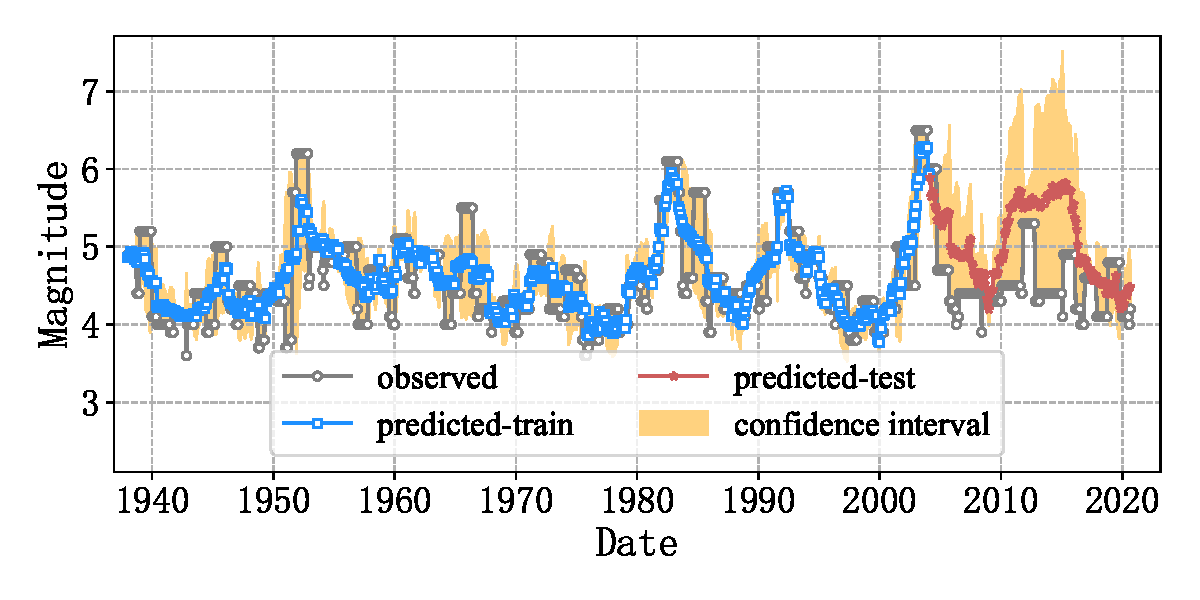
\includegraphics[width=\textwidth]{Img/chap5_seism/block2/seism_lstm_minyear_1932_maxyear_2021_spanlat_2_spanlon_4_timewindow_72_nextmonth_12_minmag_3.0_block_2.pdf}
    \vspace{-1cm}
    \label{fig:seism_lstm_minyear_1932_maxyear_2021_spanlat_2_spanlon_4_timewindow_72_nextmonth_12_minmag_3.0_block_2}
  \end{subfigure}
  ~
  \begin{subfigure}[b]{0.45\textwidth}
    \caption{SVR} 
    \vspace{-0.2cm}
    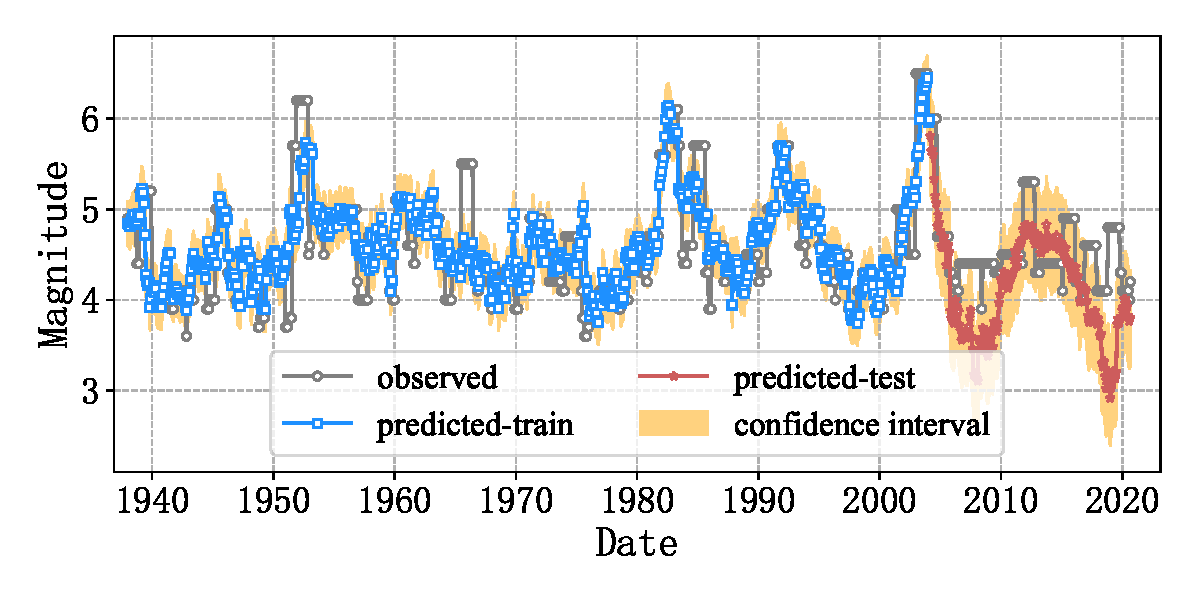
\includegraphics[width=\textwidth]{Img/chap5_seism/block2/seism_svr_minyear_1932_maxyear_2021_spanlat_2_spanlon_4_timewindow_72_nextmonth_12_minmag_3.0_block_2.pdf}
    \vspace{-1cm}
    \label{fig:seism_svr_minyear_1932_maxyear_2021_spanlat_2_spanlon_4_timewindow_72_nextmonth_12_minmag_3.0_block_2}
  \end{subfigure}   
  \\
  \begin{subfigure}[b]{0.45\textwidth}
    \caption{LR}
    \vspace{-0.2cm}
    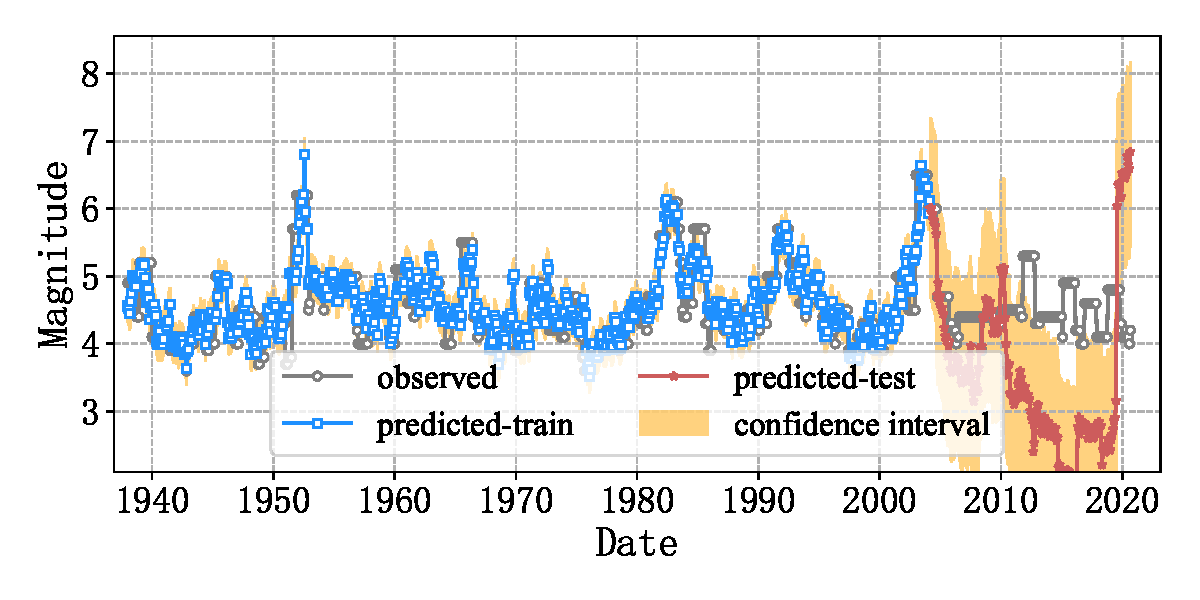
\includegraphics[width=\textwidth]{Img/chap5_seism/block2/seism_lr_minyear_1932_maxyear_2021_spanlat_2_spanlon_4_timewindow_72_nextmonth_12_minmag_3.0_block_2.pdf}
    \vspace{-1cm}
    \label{fig:seism_lr_minyear_1932_maxyear_2021_spanlat_2_spanlon_4_timewindow_72_nextmonth_12_minmag_3.0_block_2}
  \end{subfigure}
  ~
  \begin{subfigure}[b]{0.45\textwidth}
    \caption{RF}
    \vspace{-0.2cm}
    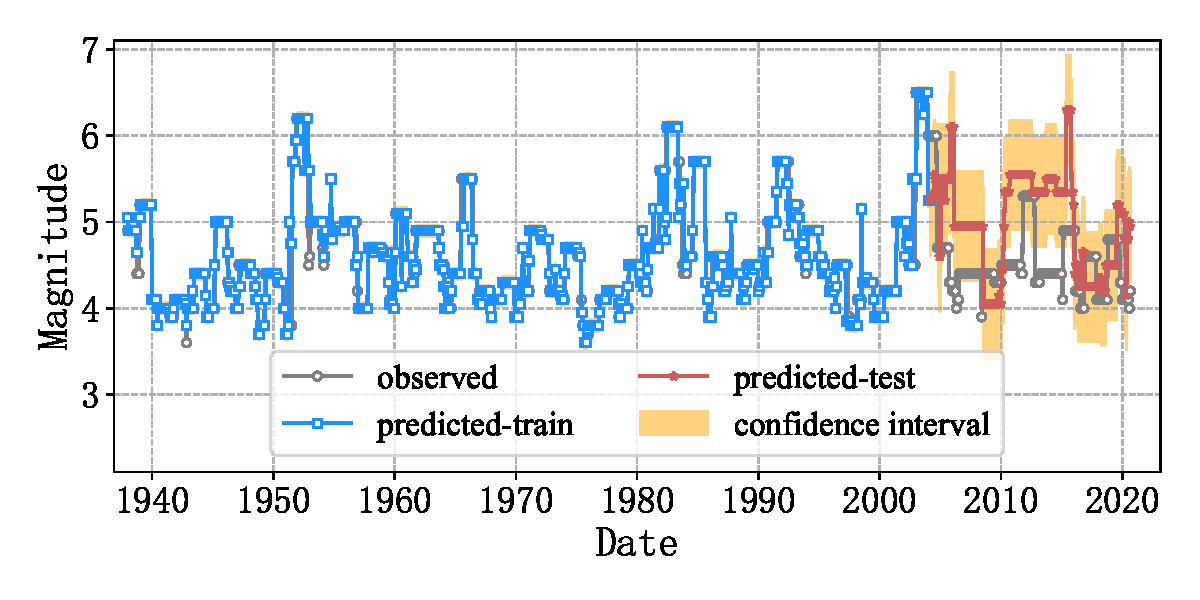
\includegraphics[width=\textwidth]{Img/chap5_seism/block2/seism_rf_minyear_1932_maxyear_2021_spanlat_2_spanlon_4_timewindow_72_nextmonth_12_minmag_3.0_block_2.pdf}
    \vspace{-1cm}
    \label{fig:seism_rf_minyear_1932_maxyear_2021_spanlat_2_spanlon_4_timewindow_72_nextmonth_12_minmag_3.0_block_2}
  \end{subfigure}
  \\
  \begin{subfigure}[b]{0.45\textwidth}
    \caption{GBRT}
    \vspace{-0.2cm}
    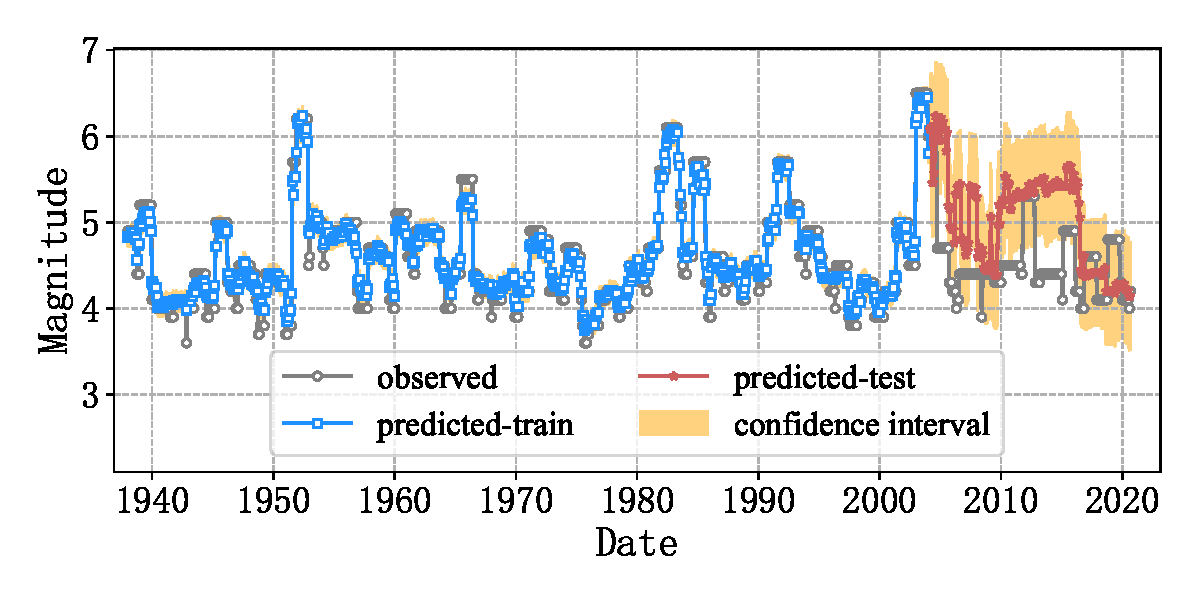
\includegraphics[width=\textwidth]{Img/chap5_seism/block2/seism_gbr_minyear_1932_maxyear_2021_spanlat_2_spanlon_4_timewindow_72_nextmonth_12_minmag_3.0_block_2.pdf}
    \vspace{-1cm}
    \label{fig:seism_gbr_minyear_1932_maxyear_2021_spanlat_2_spanlon_4_timewindow_72_nextmonth_12_minmag_3.0_block_2}
  \end{subfigure}
  ~
  \begin{subfigure}[b]{0.45\textwidth}
    \caption{DT}
    \vspace{-0.2cm}
    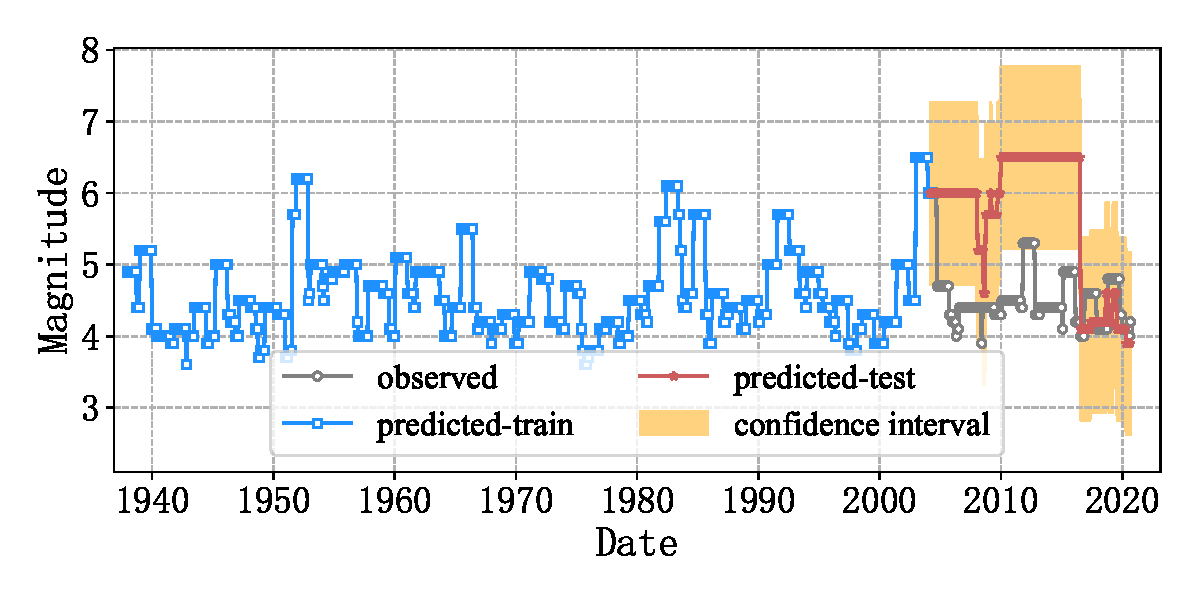
\includegraphics[width=\textwidth]{Img/chap5_seism/block2/seism_dt_minyear_1932_maxyear_2021_spanlat_2_spanlon_4_timewindow_72_nextmonth_12_minmag_3.0_block_2.pdf}
    \vspace{-1cm}
    \label{fig:seism_dt_minyear_1932_maxyear_2021_spanlat_2_spanlon_4_timewindow_72_nextmonth_12_minmag_3.0_block_2}
  \end{subfigure}
  \\
  \begin{subfigure}[b]{0.45\textwidth}
    \caption{KNN}
    \vspace{-0.2cm}
    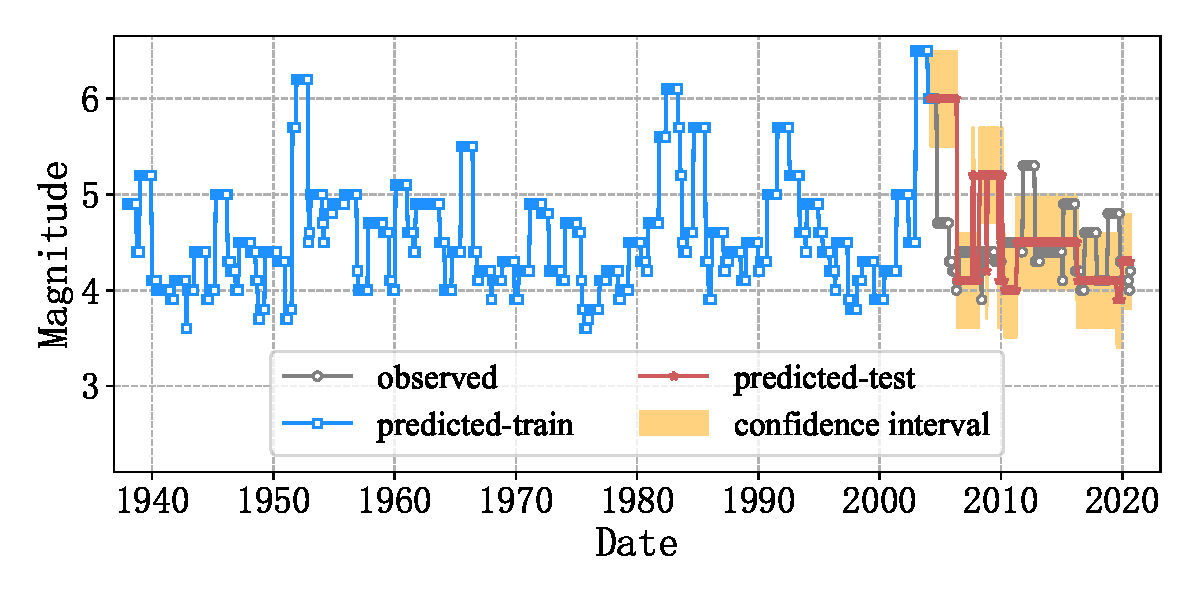
\includegraphics[width=\textwidth]{Img/chap5_seism/block2/seism_kn_minyear_1932_maxyear_2021_spanlat_2_spanlon_4_timewindow_72_nextmonth_12_minmag_3.0_block_2.pdf}
    \vspace{-1cm}
    \label{fig:seism_knn_minyear_1932_maxyear_2021_spanlat_2_spanlon_4_timewindow_72_nextmonth_12_minmag_3.0_block_2}
  \end{subfigure}
  ~
  \begin{subfigure}[b]{0.45\textwidth}
    \caption{ETR}
    \vspace{-0.2cm}
    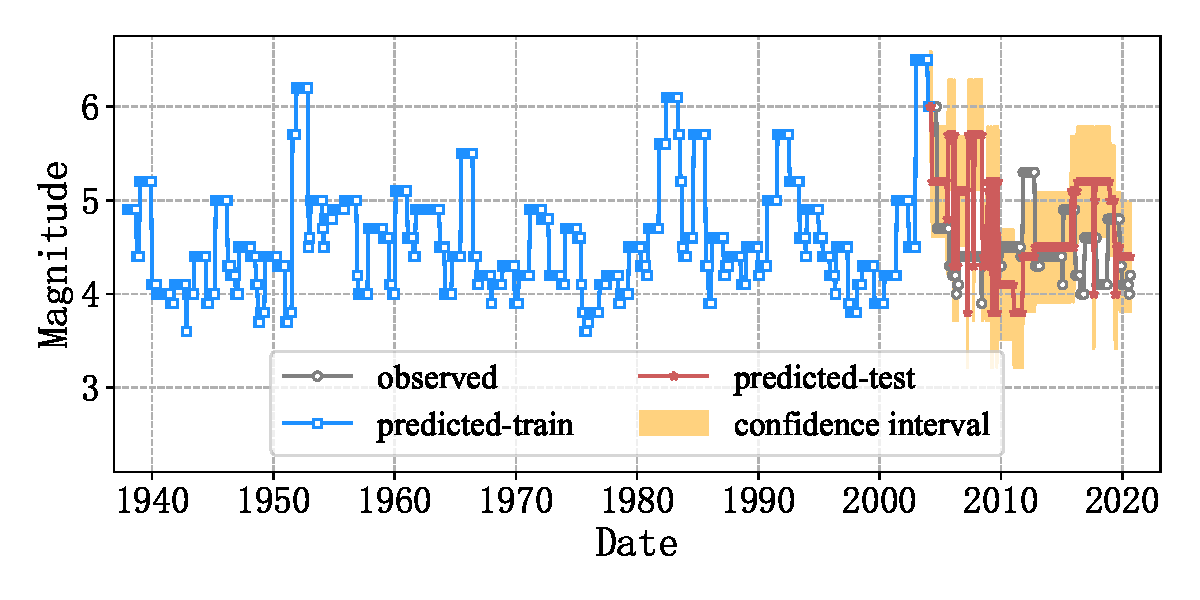
\includegraphics[width=\textwidth]{Img/chap5_seism/block2/seism_etr_minyear_1932_maxyear_2021_spanlat_2_spanlon_4_timewindow_72_nextmonth_12_minmag_3.0_block_2.pdf}
    \vspace{-1cm}
    \label{fig:seism_etr_minyear_1932_maxyear_2021_spanlat_2_spanlon_4_timewindow_72_nextmonth_12_minmag_3.0_block_2}
  \end{subfigure}
  \bicaption[不同模型预测区块2未来1年最大震级的时间序列图(数据集划分比例为0.8:0.2)]{不同模型预测区块2未来1年最大震级的时间序列图(数据集划分比例为0.8:0.2)。}{The time series of predicting the maximum magnitute of block 2 with the split ratio 0.8:0.2 in next year by different models.}
  \label{fig:seism_minyear_1932_maxyear_2021_spanlat_2_spanlon_4_timewindow_72_nextmonth_12_minmag_3.0_block_2}
\end{figure}

\begin{figure}[!htbp]
  \centering
  \begin{subfigure}[b]{0.45\textwidth}
    \caption{LSTM}
    \vspace{-0.2cm}
    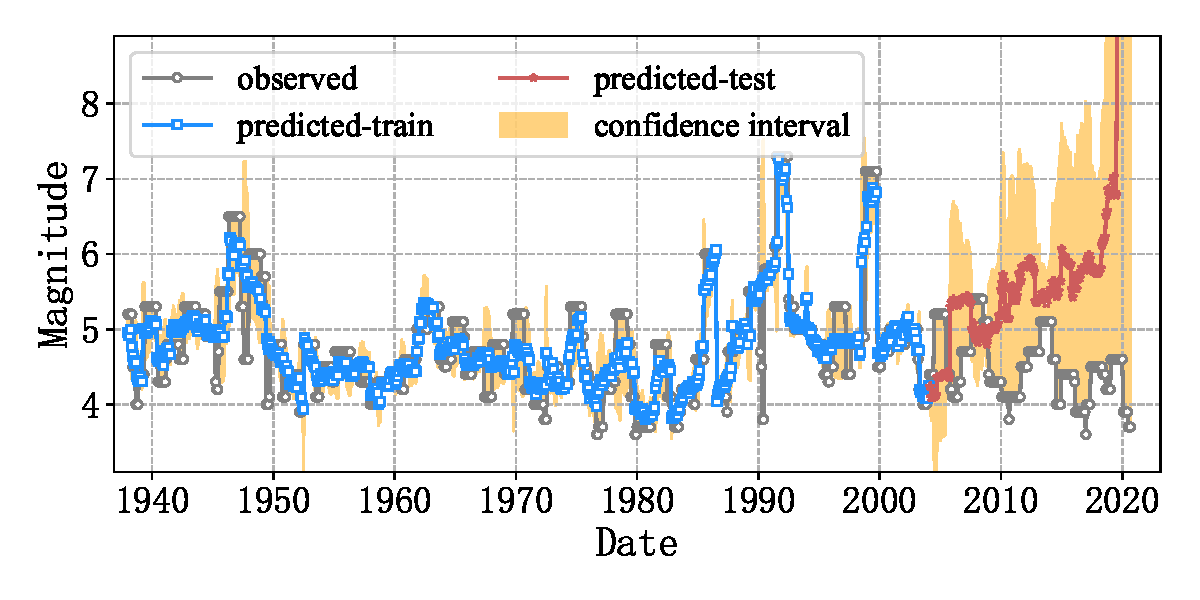
\includegraphics[width=\textwidth]{Img/chap5_seism/block3/seism_lstm_minyear_1932_maxyear_2021_spanlat_2_spanlon_4_timewindow_72_nextmonth_12_minmag_3.0_block_3.pdf}
    \vspace{-1cm}
    \label{fig:seism_lstm_minyear_1932_maxyear_2021_spanlat_2_spanlon_4_timewindow_72_nextmonth_12_minmag_3.0_block_3}
  \end{subfigure}
  ~
  \begin{subfigure}[b]{0.45\textwidth}
    \caption{SVR} 
    \vspace{-0.2cm}
    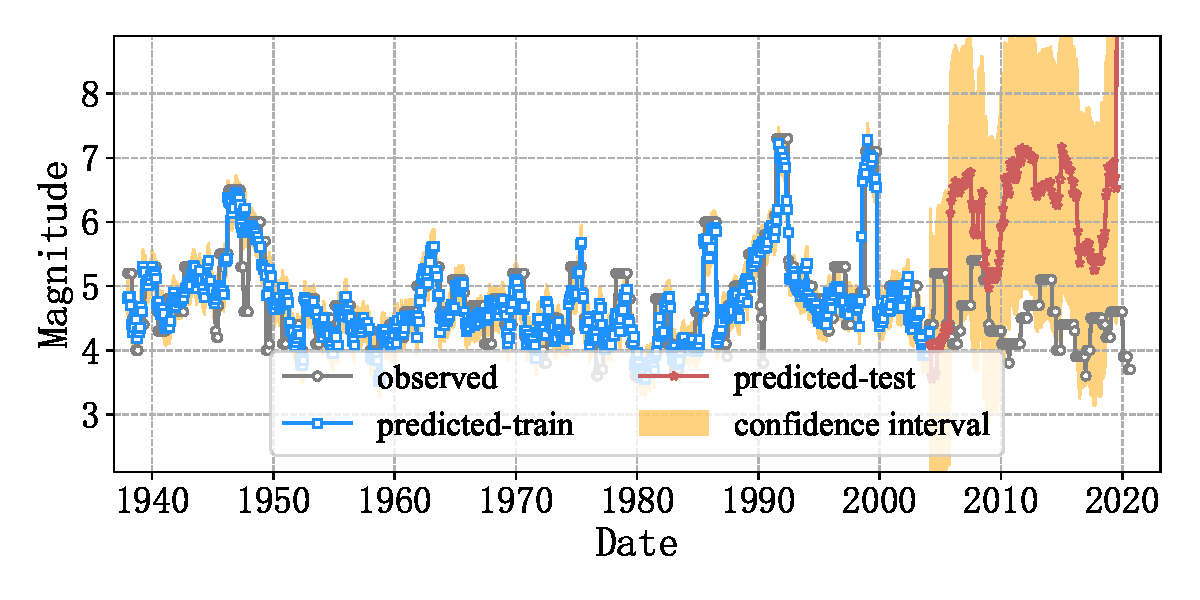
\includegraphics[width=\textwidth]{Img/chap5_seism/block3/seism_svr_minyear_1932_maxyear_2021_spanlat_2_spanlon_4_timewindow_72_nextmonth_12_minmag_3.0_block_3.pdf}
    \vspace{-1cm}
    \label{fig:seism_svr_minyear_1932_maxyear_2021_spanlat_2_spanlon_4_timewindow_72_nextmonth_12_minmag_3.0_block_3}
  \end{subfigure}   
  \\
  \begin{subfigure}[b]{0.45\textwidth}
    \caption{LR}
    \vspace{-0.2cm}
    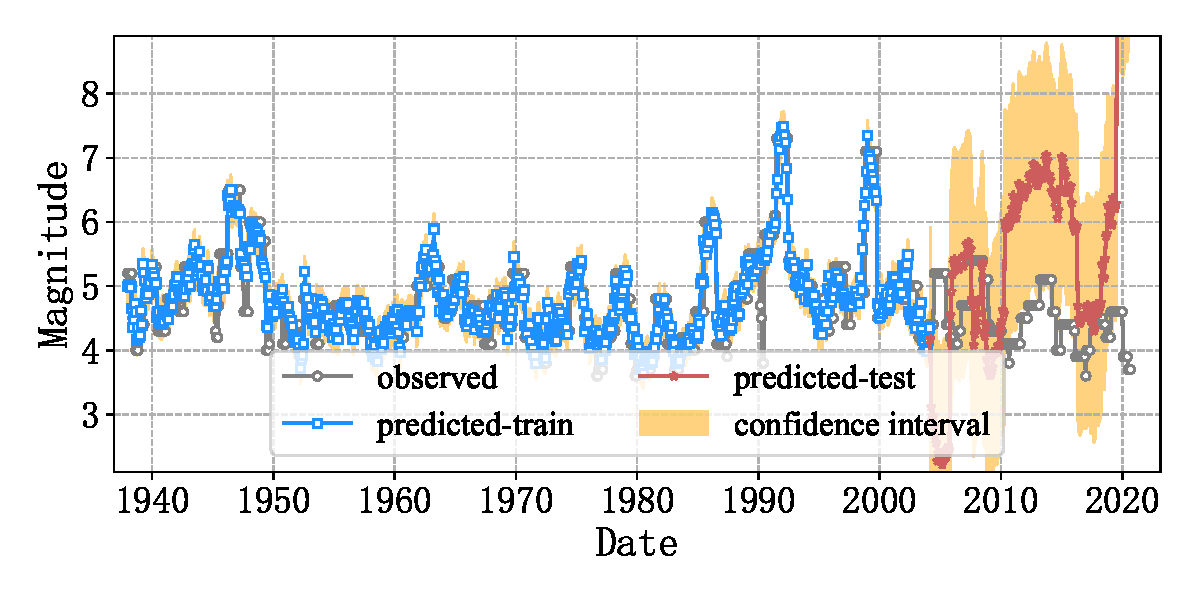
\includegraphics[width=\textwidth]{Img/chap5_seism/block3/seism_lr_minyear_1932_maxyear_2021_spanlat_2_spanlon_4_timewindow_72_nextmonth_12_minmag_3.0_block_3.pdf}
    \vspace{-1cm}
    \label{fig:seism_lr_minyear_1932_maxyear_2021_spanlat_2_spanlon_4_timewindow_72_nextmonth_12_minmag_3.0_block_3}
  \end{subfigure}
  ~
  \begin{subfigure}[b]{0.45\textwidth}
    \caption{RF}
    \vspace{-0.2cm}
    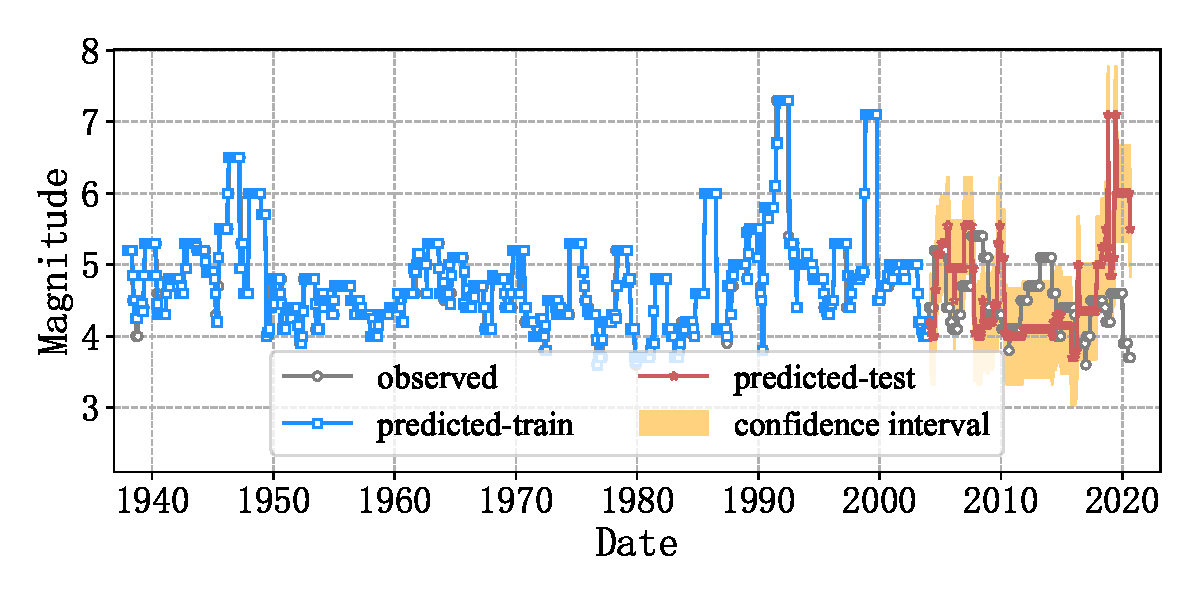
\includegraphics[width=\textwidth]{Img/chap5_seism/block3/seism_rf_minyear_1932_maxyear_2021_spanlat_2_spanlon_4_timewindow_72_nextmonth_12_minmag_3.0_block_3.pdf}
    \vspace{-1cm}
    \label{fig:seism_rf_minyear_1932_maxyear_2021_spanlat_2_spanlon_4_timewindow_72_nextmonth_12_minmag_3.0_block_3}
  \end{subfigure}
  \\
  \begin{subfigure}[b]{0.45\textwidth}
    \caption{GBRT}
    \vspace{-0.2cm}
    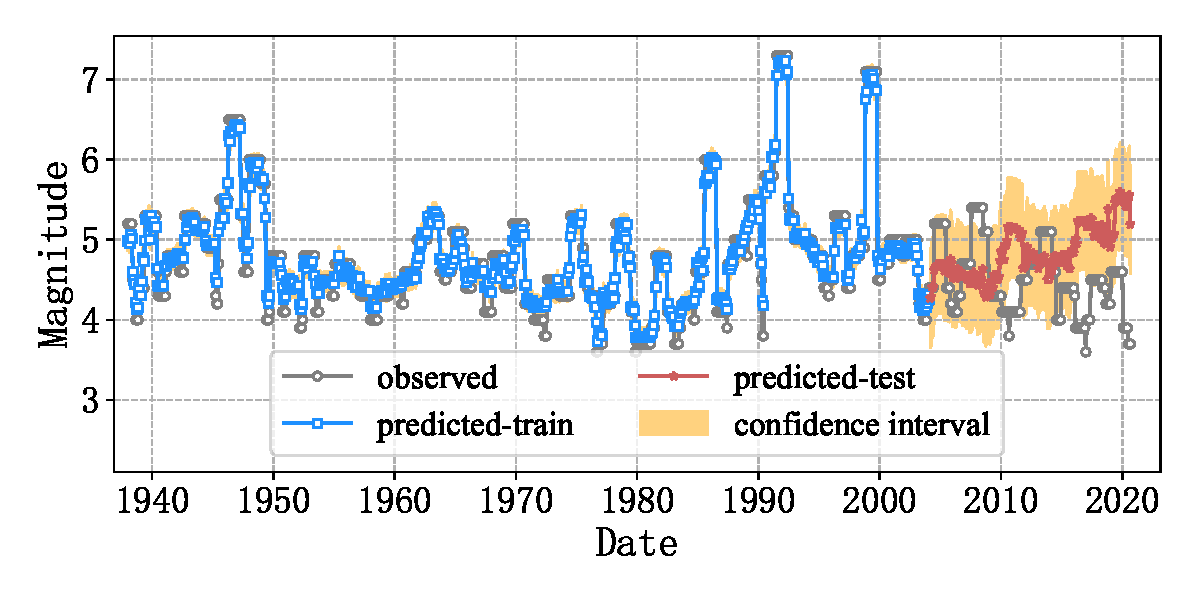
\includegraphics[width=\textwidth]{Img/chap5_seism/block3/seism_gbr_minyear_1932_maxyear_2021_spanlat_2_spanlon_4_timewindow_72_nextmonth_12_minmag_3.0_block_3.pdf}
    \vspace{-1cm}
    \label{fig:seism_gbr_minyear_1932_maxyear_2021_spanlat_2_spanlon_4_timewindow_72_nextmonth_12_minmag_3.0_block_3}
  \end{subfigure}
  ~
  \begin{subfigure}[b]{0.45\textwidth}
    \caption{DT}
    \vspace{-0.2cm}
    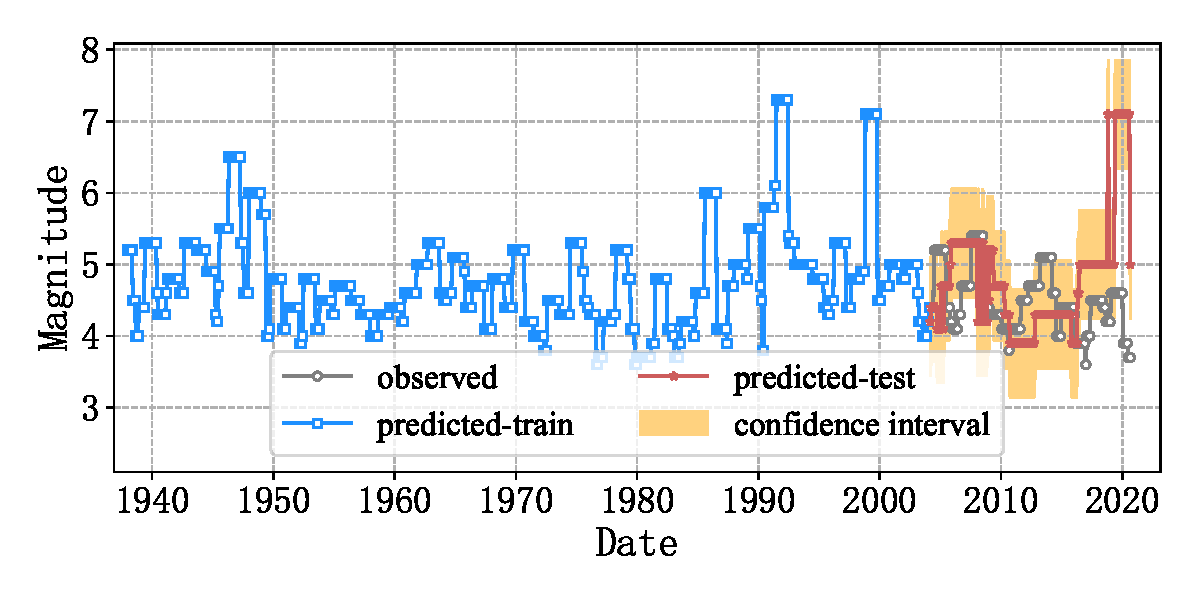
\includegraphics[width=\textwidth]{Img/chap5_seism/block3/seism_dt_minyear_1932_maxyear_2021_spanlat_2_spanlon_4_timewindow_72_nextmonth_12_minmag_3.0_block_3.pdf}
    \vspace{-1cm}
    \label{fig:seism_dt_minyear_1932_maxyear_2021_spanlat_2_spanlon_4_timewindow_72_nextmonth_12_minmag_3.0_block_3}
  \end{subfigure}
  \\
  \begin{subfigure}[b]{0.45\textwidth}
    \caption{KNN}
    \vspace{-0.2cm}
    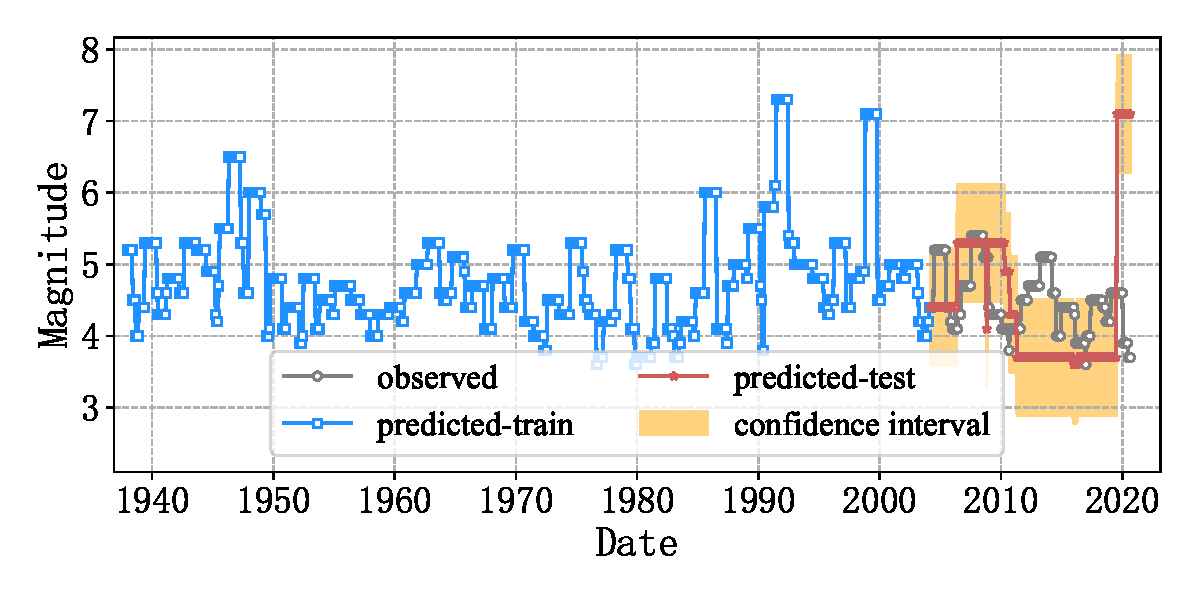
\includegraphics[width=\textwidth]{Img/chap5_seism/block3/seism_kn_minyear_1932_maxyear_2021_spanlat_2_spanlon_4_timewindow_72_nextmonth_12_minmag_3.0_block_3.pdf}
    \vspace{-1cm}
    \label{fig:seism_knn_minyear_1932_maxyear_2021_spanlat_2_spanlon_4_timewindow_72_nextmonth_12_minmag_3.0_block_3}
  \end{subfigure}
  ~
  \begin{subfigure}[b]{0.45\textwidth}
    \caption{ETR}
    \vspace{-0.2cm}
    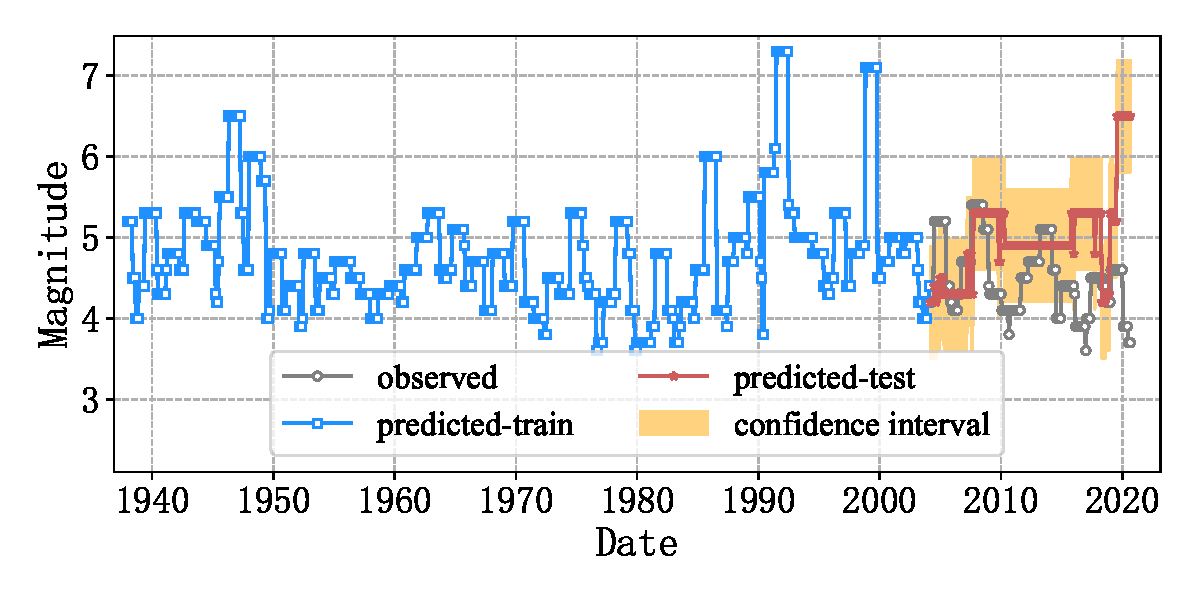
\includegraphics[width=\textwidth]{Img/chap5_seism/block3/seism_etr_minyear_1932_maxyear_2021_spanlat_2_spanlon_4_timewindow_72_nextmonth_12_minmag_3.0_block_3.pdf}
    \vspace{-1cm}
    \label{fig:seism_etr_minyear_1932_maxyear_2021_spanlat_2_spanlon_4_timewindow_72_nextmonth_12_minmag_3.0_block_3}
  \end{subfigure}
  \bicaption[不同模型预测区块3未来1年最大震级的时间序列图(数据集划分比例为0.8:0.2)]{不同模型预测区块3未来1年最大震级的时间序列图(数据集划分比例为0.8:0.2)。}{The time series of predicting the maximum magnitute of block 3 with the split ratio 0.8:0.2 in next year by different models.}
  \label{fig:seism_minyear_1932_maxyear_2021_spanlat_2_spanlon_4_timewindow_72_nextmonth_12_minmag_3.0_block_3}
\end{figure}

\begin{figure}[!htbp]
  \centering
  \begin{subfigure}[b]{0.45\textwidth}
    \caption{LSTM}
    \vspace{-0.2cm}
    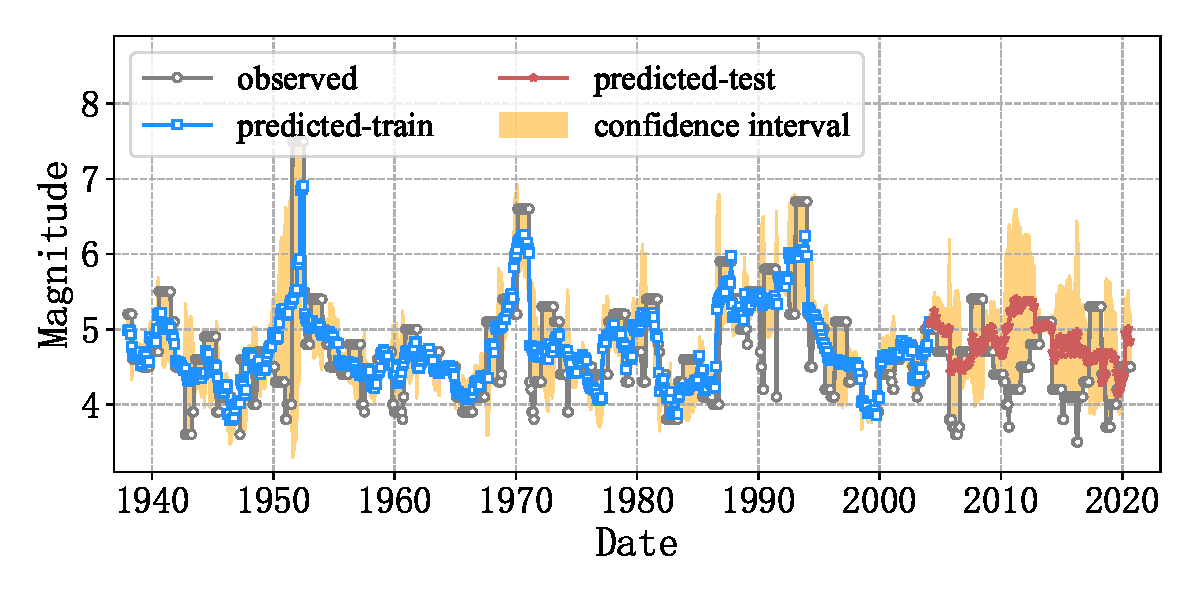
\includegraphics[width=\textwidth]{Img/chap5_seism/block4/seism_lstm_minyear_1932_maxyear_2021_spanlat_2_spanlon_4_timewindow_72_nextmonth_12_minmag_3.0_block_4.pdf}
    \vspace{-1cm}
    \label{fig:seism_lstm_minyear_1932_maxyear_2021_spanlat_2_spanlon_4_timewindow_72_nextmonth_12_minmag_3.0_block_4}
  \end{subfigure}
  ~
  \begin{subfigure}[b]{0.45\textwidth}
    \caption{SVR} 
    \vspace{-0.2cm}
    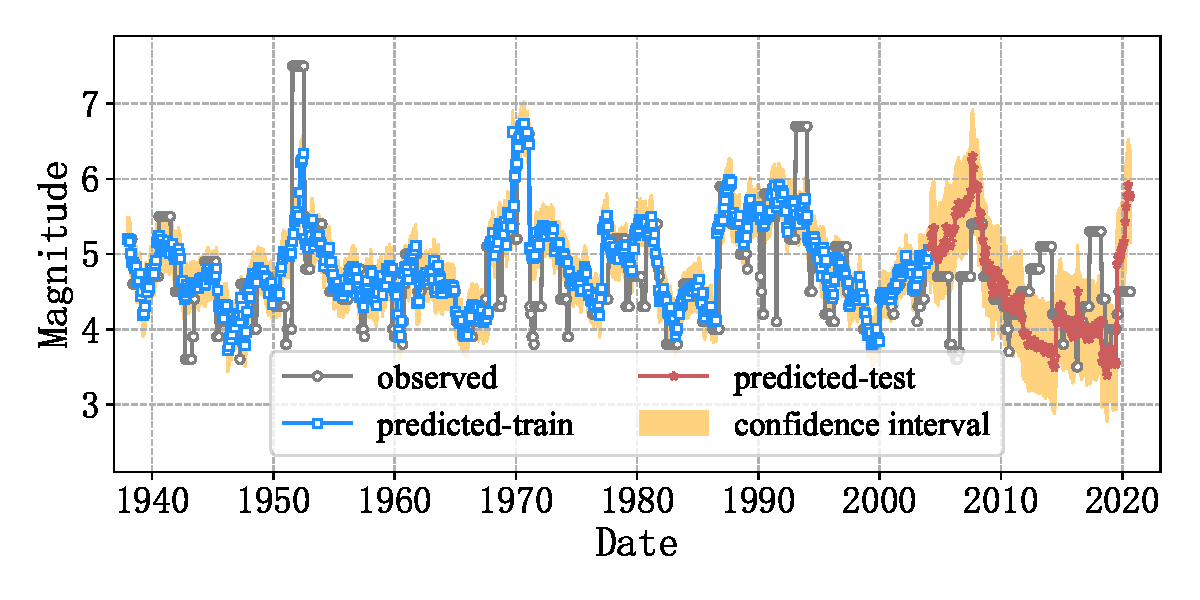
\includegraphics[width=\textwidth]{Img/chap5_seism/block4/seism_svr_minyear_1932_maxyear_2021_spanlat_2_spanlon_4_timewindow_72_nextmonth_12_minmag_3.0_block_4.pdf}
    \vspace{-1cm}
    \label{fig:seism_svr_minyear_1932_maxyear_2021_spanlat_2_spanlon_4_timewindow_72_nextmonth_12_minmag_3.0_block_4}
  \end{subfigure}   
  \\
  \begin{subfigure}[b]{0.45\textwidth}
    \caption{LR}
    \vspace{-0.2cm}
    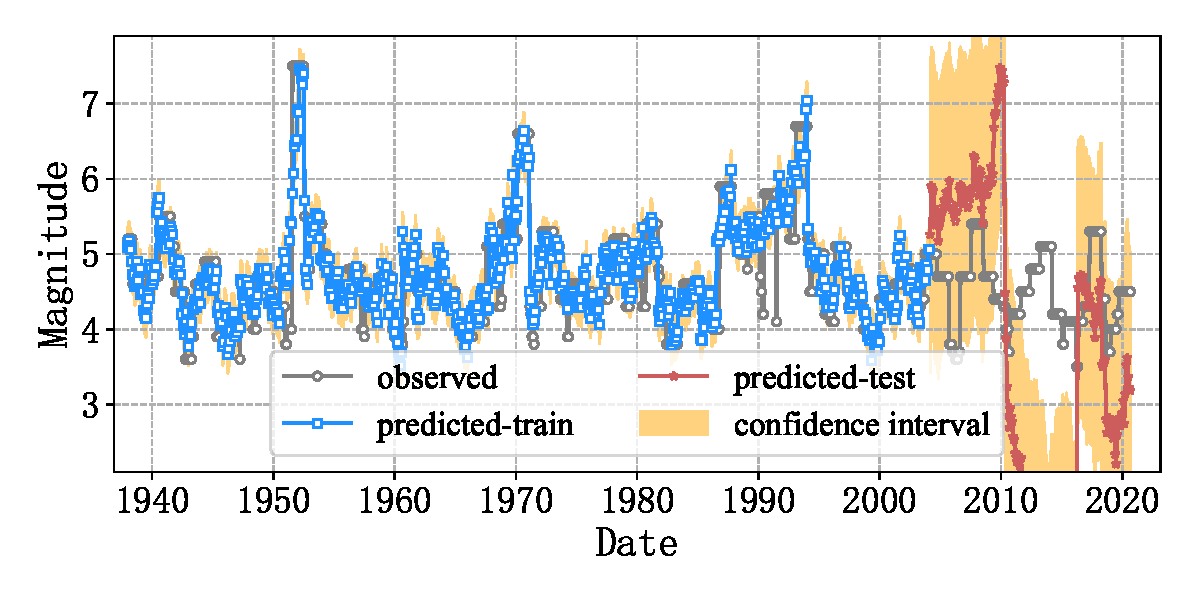
\includegraphics[width=\textwidth]{Img/chap5_seism/block4/seism_lr_minyear_1932_maxyear_2021_spanlat_2_spanlon_4_timewindow_72_nextmonth_12_minmag_3.0_block_4.pdf}
    \vspace{-1cm}
    \label{fig:seism_lr_minyear_1932_maxyear_2021_spanlat_2_spanlon_4_timewindow_72_nextmonth_12_minmag_3.0_block_4}
  \end{subfigure}
  ~
  \begin{subfigure}[b]{0.45\textwidth}
    \caption{RF}
    \vspace{-0.2cm}
    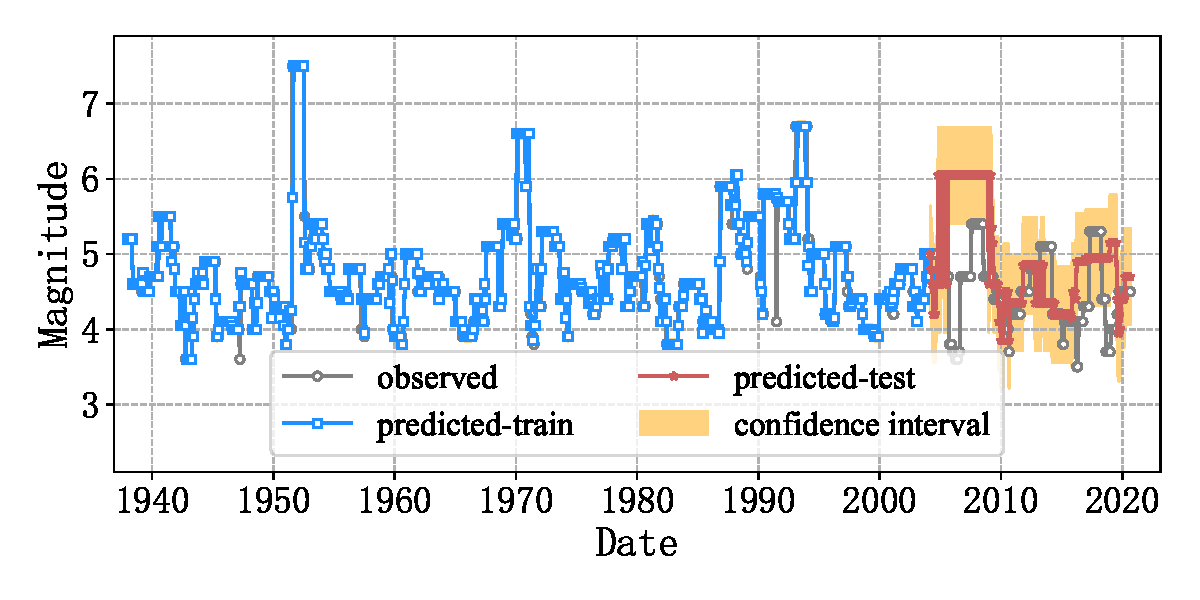
\includegraphics[width=\textwidth]{Img/chap5_seism/block4/seism_rf_minyear_1932_maxyear_2021_spanlat_2_spanlon_4_timewindow_72_nextmonth_12_minmag_3.0_block_4.pdf}
    \vspace{-1cm}
    \label{fig:seism_rf_minyear_1932_maxyear_2021_spanlat_2_spanlon_4_timewindow_72_nextmonth_12_minmag_3.0_block_4}
  \end{subfigure}
  \\
  \begin{subfigure}[b]{0.45\textwidth}
    \caption{GBRT}
    \vspace{-0.2cm}
    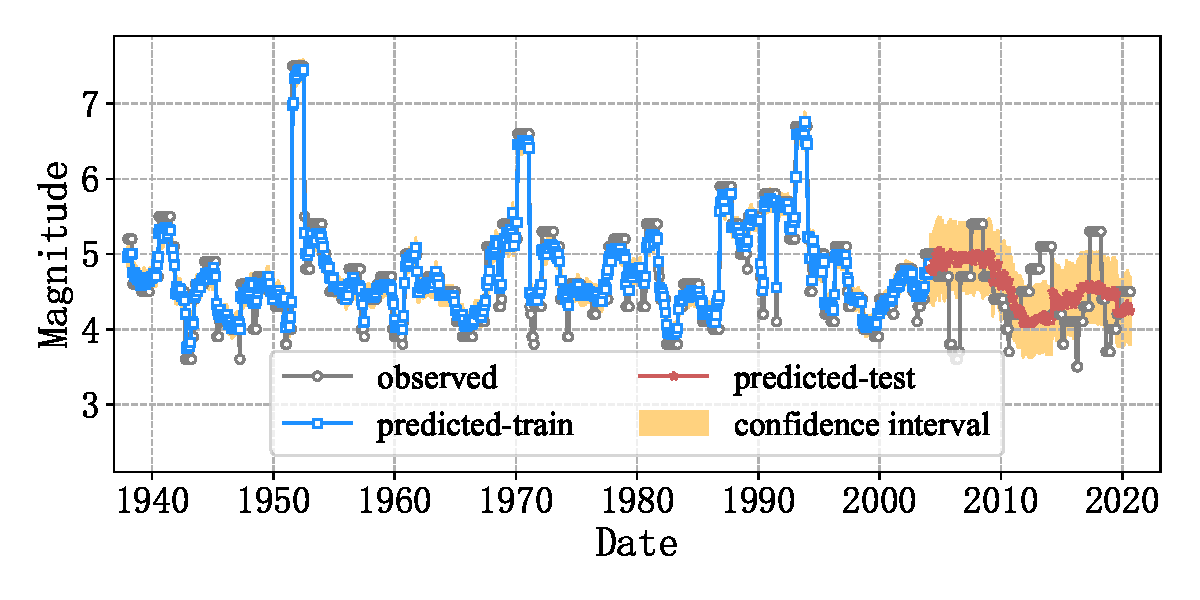
\includegraphics[width=\textwidth]{Img/chap5_seism/block4/seism_gbr_minyear_1932_maxyear_2021_spanlat_2_spanlon_4_timewindow_72_nextmonth_12_minmag_3.0_block_4.pdf}
    \vspace{-1cm}
    \label{fig:seism_gbr_minyear_1932_maxyear_2021_spanlat_2_spanlon_4_timewindow_72_nextmonth_12_minmag_3.0_block_4}
  \end{subfigure}
  ~
  \begin{subfigure}[b]{0.45\textwidth}
    \caption{DT}
    \vspace{-0.2cm}
    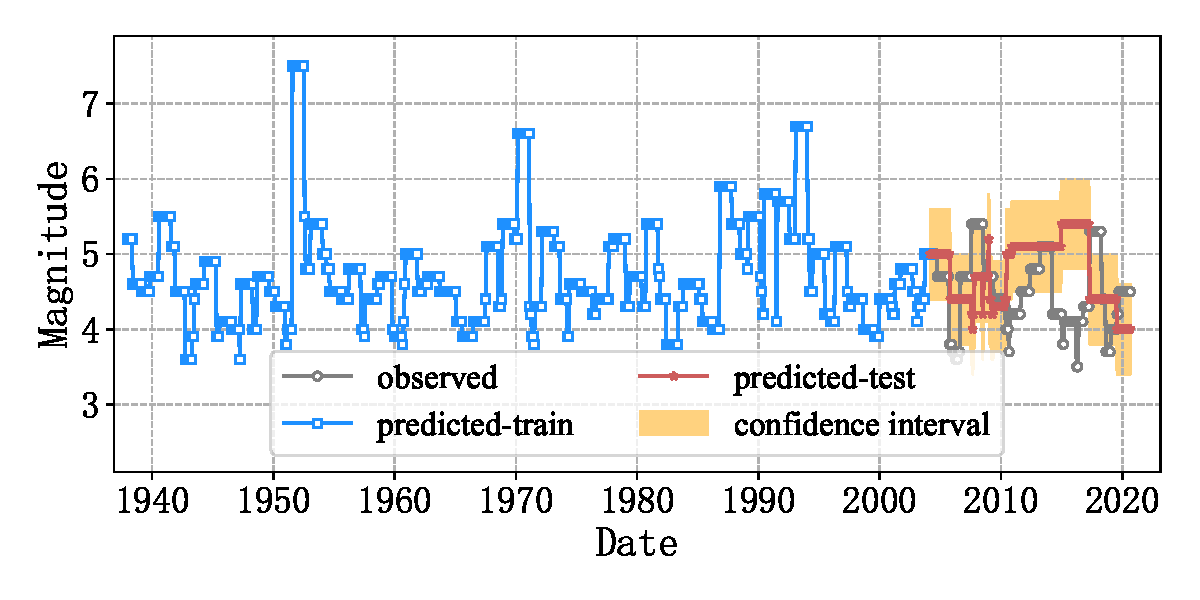
\includegraphics[width=\textwidth]{Img/chap5_seism/block4/seism_dt_minyear_1932_maxyear_2021_spanlat_2_spanlon_4_timewindow_72_nextmonth_12_minmag_3.0_block_4.pdf}
    \vspace{-1cm}
    \label{fig:seism_dt_minyear_1932_maxyear_2021_spanlat_2_spanlon_4_timewindow_72_nextmonth_12_minmag_3.0_block_4}
  \end{subfigure}
  \\
  \begin{subfigure}[b]{0.45\textwidth}
    \caption{KNN}
    \vspace{-0.2cm}
    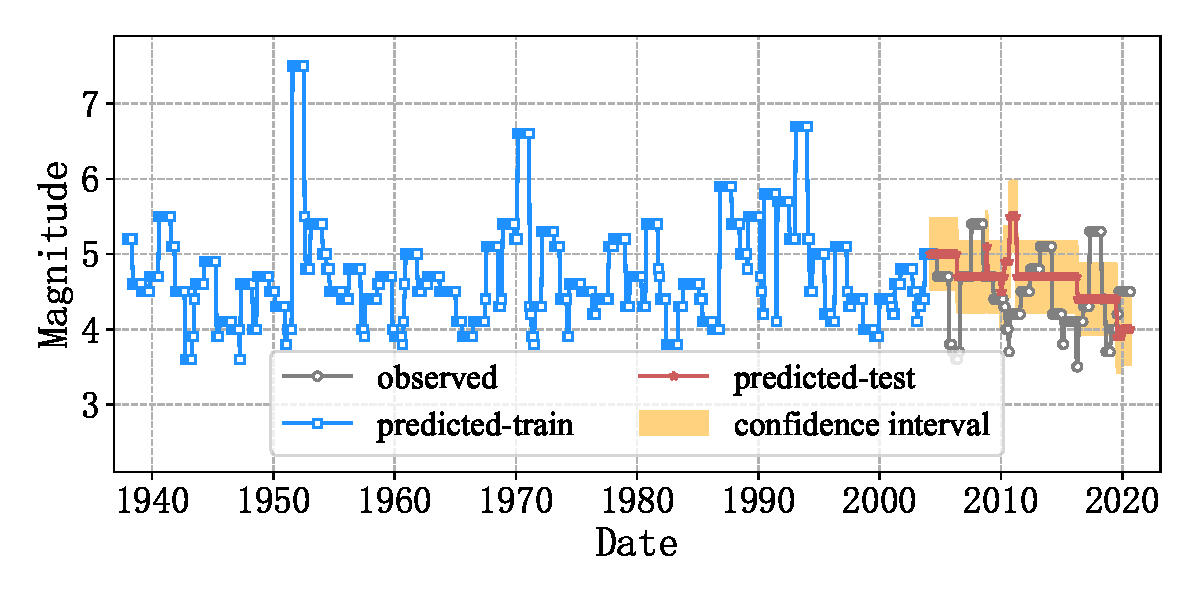
\includegraphics[width=\textwidth]{Img/chap5_seism/block4/seism_kn_minyear_1932_maxyear_2021_spanlat_2_spanlon_4_timewindow_72_nextmonth_12_minmag_3.0_block_4.pdf}
    \vspace{-1cm}
    \label{fig:seism_knn_minyear_1932_maxyear_2021_spanlat_2_spanlon_4_timewindow_72_nextmonth_12_minmag_3.0_block_4}
  \end{subfigure}
  ~
  \begin{subfigure}[b]{0.45\textwidth}
    \caption{ETR}
    \vspace{-0.2cm}
    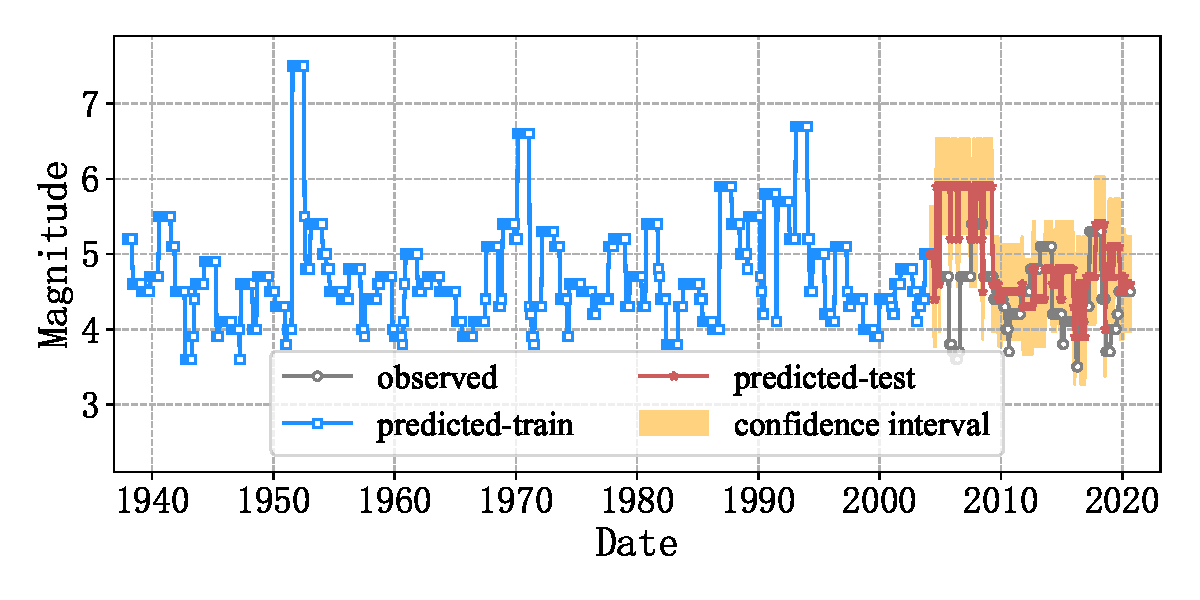
\includegraphics[width=\textwidth]{Img/chap5_seism/block4/seism_etr_minyear_1932_maxyear_2021_spanlat_2_spanlon_4_timewindow_72_nextmonth_12_minmag_3.0_block_4.pdf}
    \vspace{-1cm}
    \label{fig:seism_etr_minyear_1932_maxyear_2021_spanlat_2_spanlon_4_timewindow_72_nextmonth_12_minmag_3.0_block_4}
  \end{subfigure}
  \bicaption[不同模型预测区块4未来1年最大震级的时间序列图(数据集划分比例为0.8:0.2)]{不同模型预测区块4未来1年最大震级的时间序列图(数据集划分比例为0.8:0.2)。}{The time series of predicting the maximum magnitute of block 4 with the split ratio 0.8:0.2 in next year by different models.}
  \label{fig:seism_minyear_1932_maxyear_2021_spanlat_2_spanlon_4_timewindow_72_nextmonth_12_minmag_3.0_block_4}
\end{figure}

\begin{figure}[!htbp]
  \centering
  \begin{subfigure}[b]{0.45\textwidth}
    \caption{LSTM}
    \vspace{-0.2cm}
    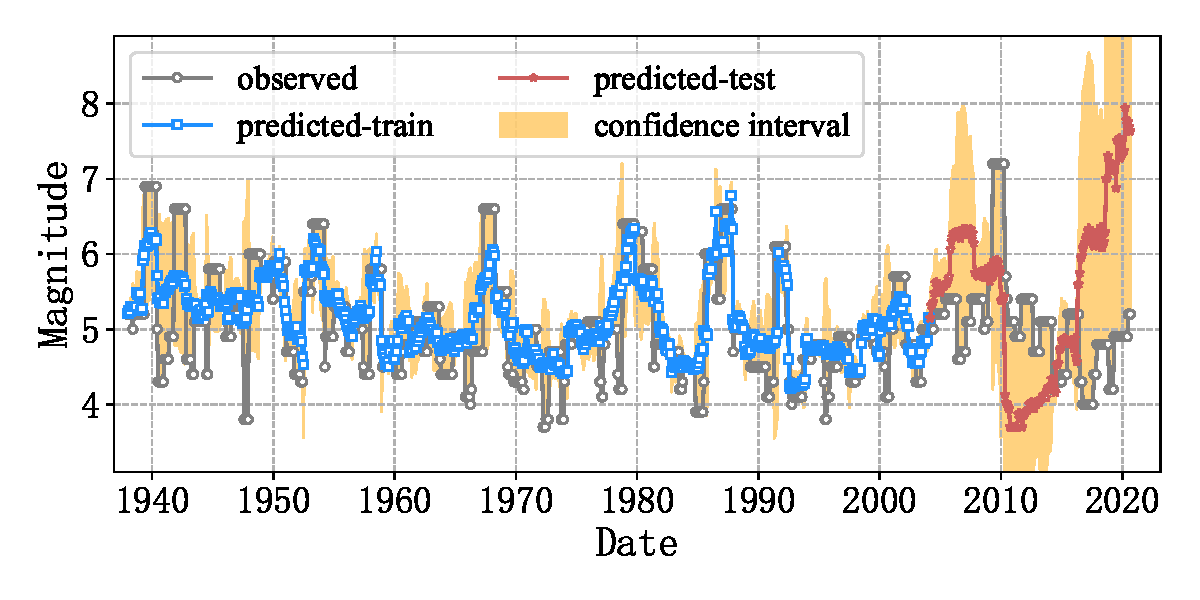
\includegraphics[width=\textwidth]{Img/chap5_seism/block5/seism_lstm_minyear_1932_maxyear_2021_spanlat_2_spanlon_4_timewindow_72_nextmonth_12_minmag_3.0_block_5.pdf}
    \vspace{-1cm}
    \label{fig:seism_lstm_minyear_1932_maxyear_2021_spanlat_2_spanlon_4_timewindow_72_nextmonth_12_minmag_3.0_block_5}
  \end{subfigure}
  ~
  \begin{subfigure}[b]{0.45\textwidth}
    \caption{SVR} 
    \vspace{-0.2cm}
    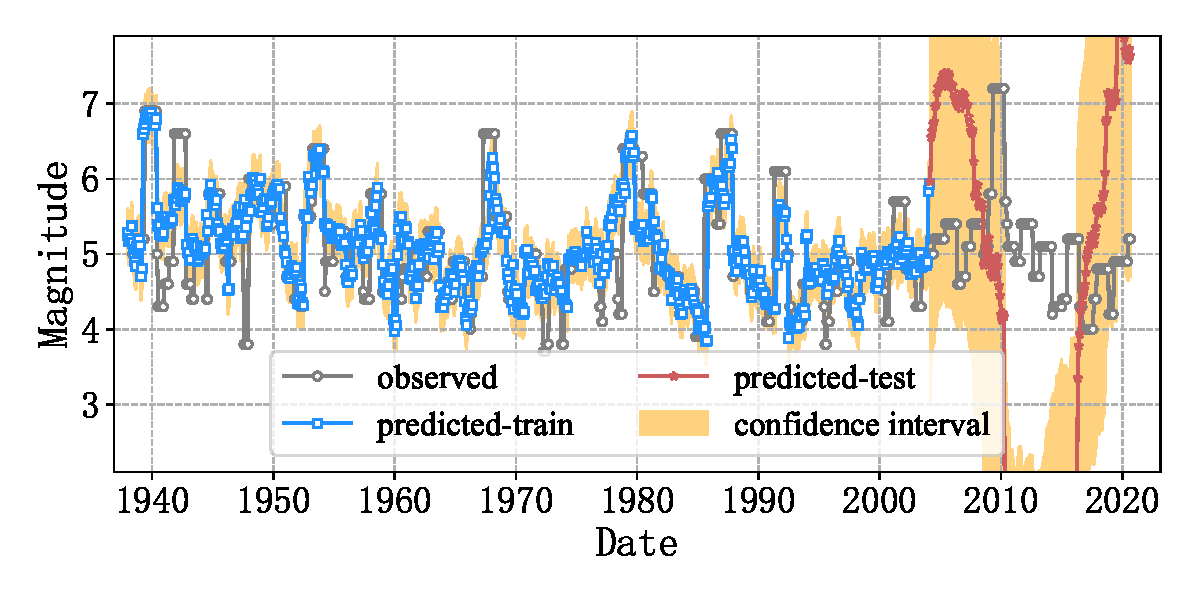
\includegraphics[width=\textwidth]{Img/chap5_seism/block5/seism_svr_minyear_1932_maxyear_2021_spanlat_2_spanlon_4_timewindow_72_nextmonth_12_minmag_3.0_block_5.pdf}
    \vspace{-1cm}
    \label{fig:seism_svr_minyear_1932_maxyear_2021_spanlat_2_spanlon_4_timewindow_72_nextmonth_12_minmag_3.0_block_5}
  \end{subfigure}   
  \\
  \begin{subfigure}[b]{0.45\textwidth}
    \caption{LR}
    \vspace{-0.2cm}
    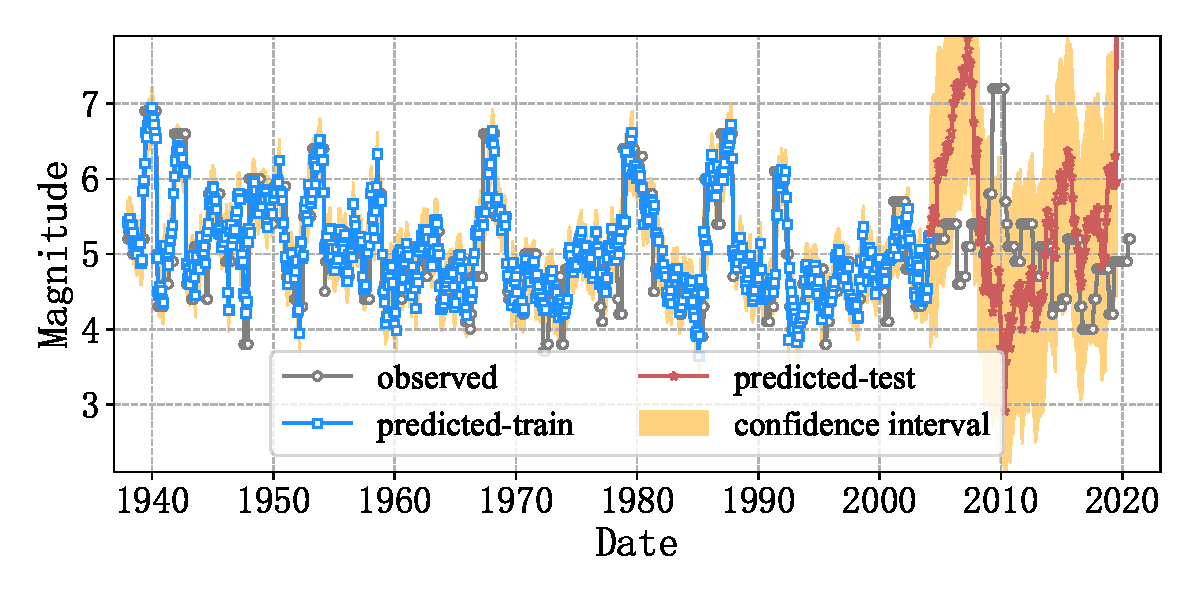
\includegraphics[width=\textwidth]{Img/chap5_seism/block5/seism_lr_minyear_1932_maxyear_2021_spanlat_2_spanlon_4_timewindow_72_nextmonth_12_minmag_3.0_block_5.pdf}
    \vspace{-1cm}
    \label{fig:seism_lr_minyear_1932_maxyear_2021_spanlat_2_spanlon_4_timewindow_72_nextmonth_12_minmag_3.0_block_5}
  \end{subfigure}
  ~
  \begin{subfigure}[b]{0.45\textwidth}
    \caption{RF}
    \vspace{-0.2cm}
    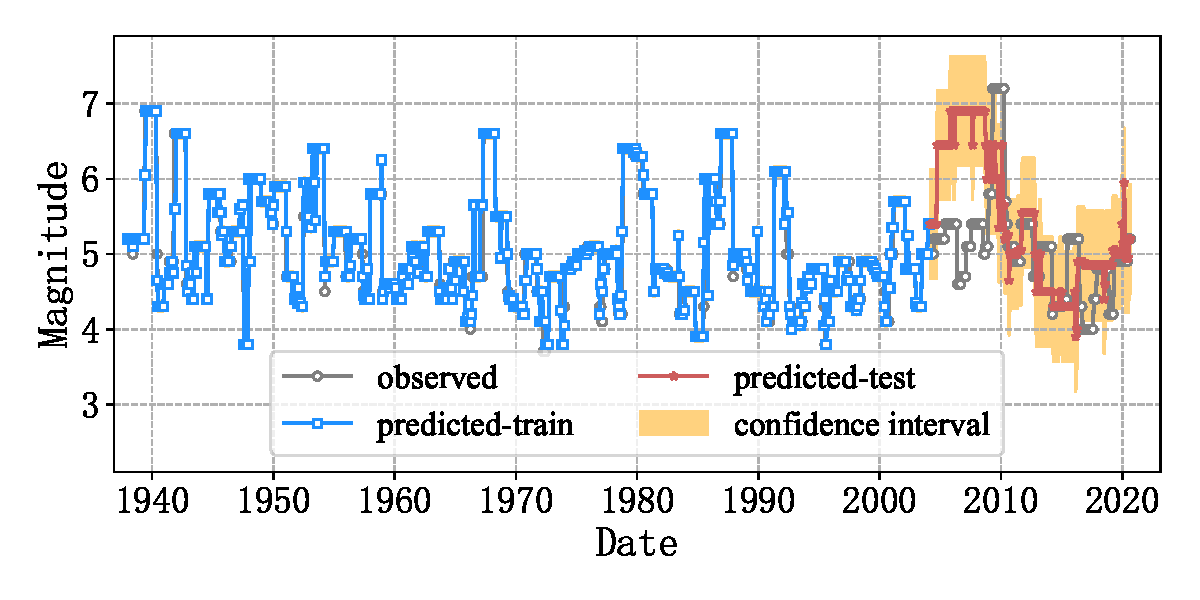
\includegraphics[width=\textwidth]{Img/chap5_seism/block5/seism_rf_minyear_1932_maxyear_2021_spanlat_2_spanlon_4_timewindow_72_nextmonth_12_minmag_3.0_block_5.pdf}
    \vspace{-1cm}
    \label{fig:seism_rf_minyear_1932_maxyear_2021_spanlat_2_spanlon_4_timewindow_72_nextmonth_12_minmag_3.0_block_5}
  \end{subfigure}
  \\
  \begin{subfigure}[b]{0.45\textwidth}
    \caption{GBRT}
    \vspace{-0.2cm}
    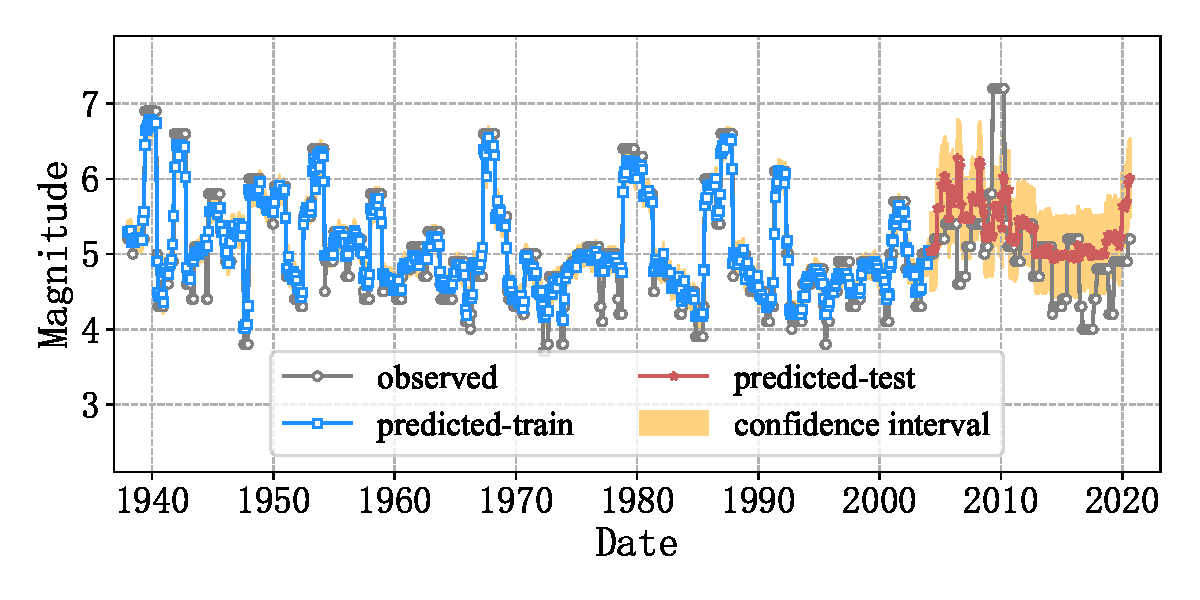
\includegraphics[width=\textwidth]{Img/chap5_seism/block5/seism_gbr_minyear_1932_maxyear_2021_spanlat_2_spanlon_4_timewindow_72_nextmonth_12_minmag_3.0_block_5.pdf}
    \vspace{-1cm}
    \label{fig:seism_gbr_minyear_1932_maxyear_2021_spanlat_2_spanlon_4_timewindow_72_nextmonth_12_minmag_3.0_block_5}
  \end{subfigure}
  ~
  \begin{subfigure}[b]{0.45\textwidth}
    \caption{DT}
    \vspace{-0.2cm}
    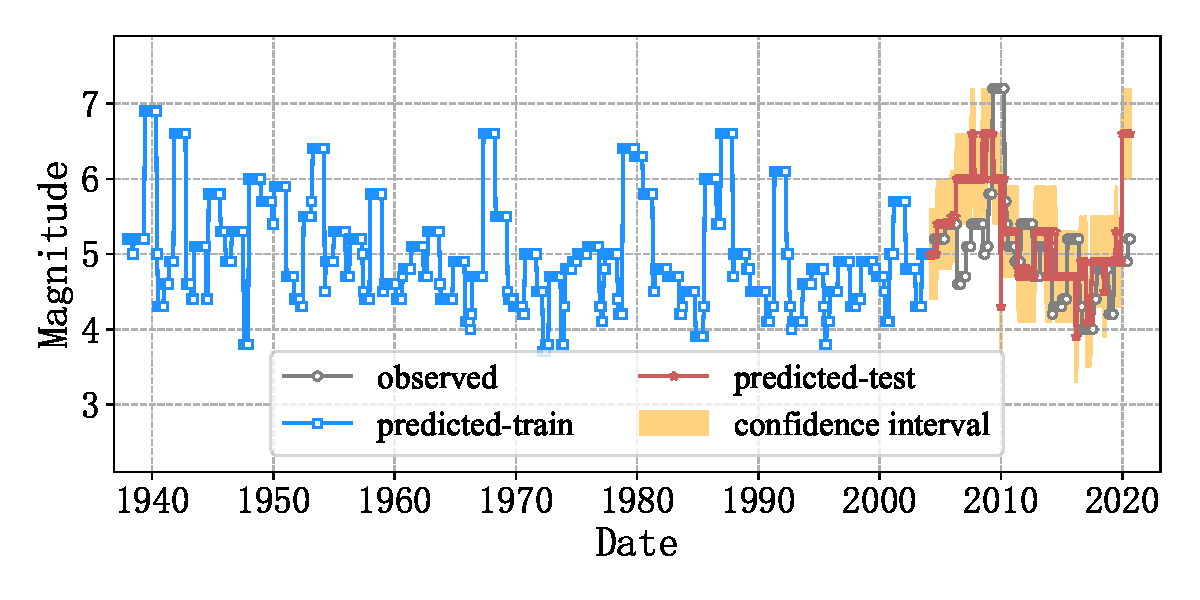
\includegraphics[width=\textwidth]{Img/chap5_seism/block5/seism_dt_minyear_1932_maxyear_2021_spanlat_2_spanlon_4_timewindow_72_nextmonth_12_minmag_3.0_block_5.pdf}
    \vspace{-1cm}
    \label{fig:seism_dt_minyear_1932_maxyear_2021_spanlat_2_spanlon_4_timewindow_72_nextmonth_12_minmag_3.0_block_5}
  \end{subfigure}
  \\
  \begin{subfigure}[b]{0.45\textwidth}
    \caption{KNN}
    \vspace{-0.2cm}
    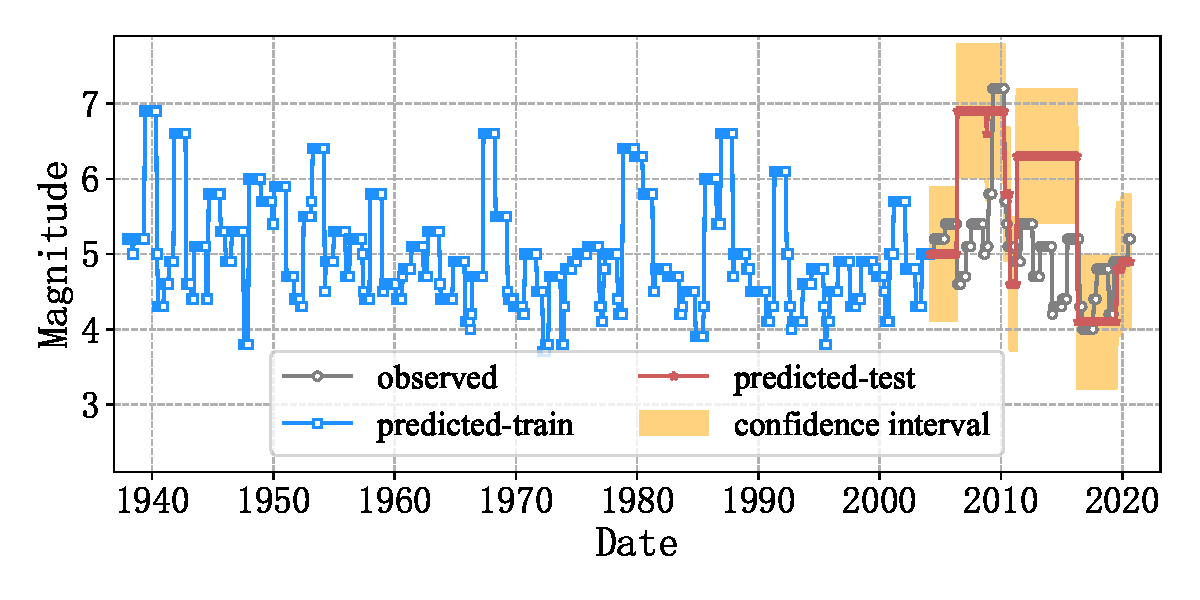
\includegraphics[width=\textwidth]{Img/chap5_seism/block5/seism_kn_minyear_1932_maxyear_2021_spanlat_2_spanlon_4_timewindow_72_nextmonth_12_minmag_3.0_block_5.pdf}
    \vspace{-1cm}
    \label{fig:seism_knn_minyear_1932_maxyear_2021_spanlat_2_spanlon_4_timewindow_72_nextmonth_12_minmag_3.0_block_5}
  \end{subfigure}
  ~
  \begin{subfigure}[b]{0.45\textwidth}
    \caption{ETR}
    \vspace{-0.2cm}
    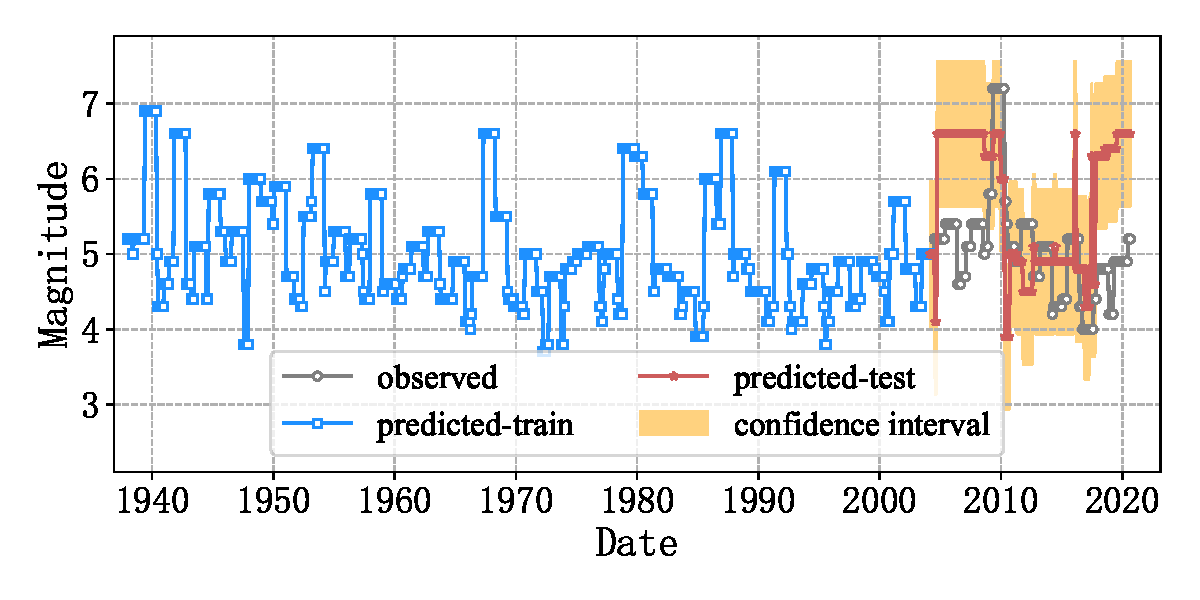
\includegraphics[width=\textwidth]{Img/chap5_seism/block5/seism_etr_minyear_1932_maxyear_2021_spanlat_2_spanlon_4_timewindow_72_nextmonth_12_minmag_3.0_block_5.pdf}
    \vspace{-1cm}
    \label{fig:seism_etr_minyear_1932_maxyear_2021_spanlat_2_spanlon_4_timewindow_72_nextmonth_12_minmag_3.0_block_5}
  \end{subfigure}
  \bicaption[不同模型预测区块5未来1年最大震级的时间序列图(数据集划分比例为0.8:0.2)]{不同模型预测区块5未来1年最大震级的时间序列图(数据集划分比例为0.8:0.2)。}{The time series of predicting the maximum magnitute of block 5 with the split ratio 0.8:0.2 in next year by different models.}
  \label{fig:seism_minyear_1932_maxyear_2021_spanlat_2_spanlon_4_timewindow_72_nextmonth_12_minmag_3.0_block_5}
\end{figure}

\begin{figure}[!htbp]
  \centering
  \begin{subfigure}[b]{0.45\textwidth}
    \caption{LSTM}
    \vspace{-0.2cm}
    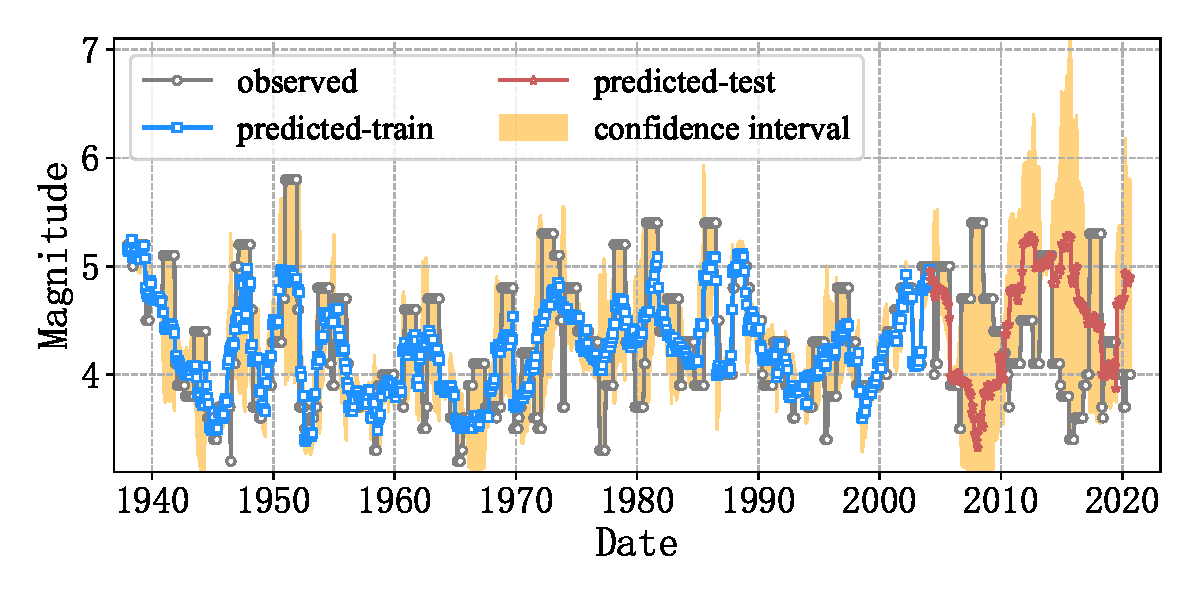
\includegraphics[width=\textwidth]{Img/chap5_seism/block6/seism_lstm_minyear_1932_maxyear_2021_spanlat_2_spanlon_4_timewindow_72_nextmonth_12_minmag_3.0_block_6.pdf}
    \vspace{-1cm}
    \label{fig:seism_lstm_minyear_1932_maxyear_2021_spanlat_2_spanlon_4_timewindow_72_nextmonth_12_minmag_3.0_block_6}
  \end{subfigure}
  ~
  \begin{subfigure}[b]{0.45\textwidth}
    \caption{SVR} 
    \vspace{-0.2cm}
    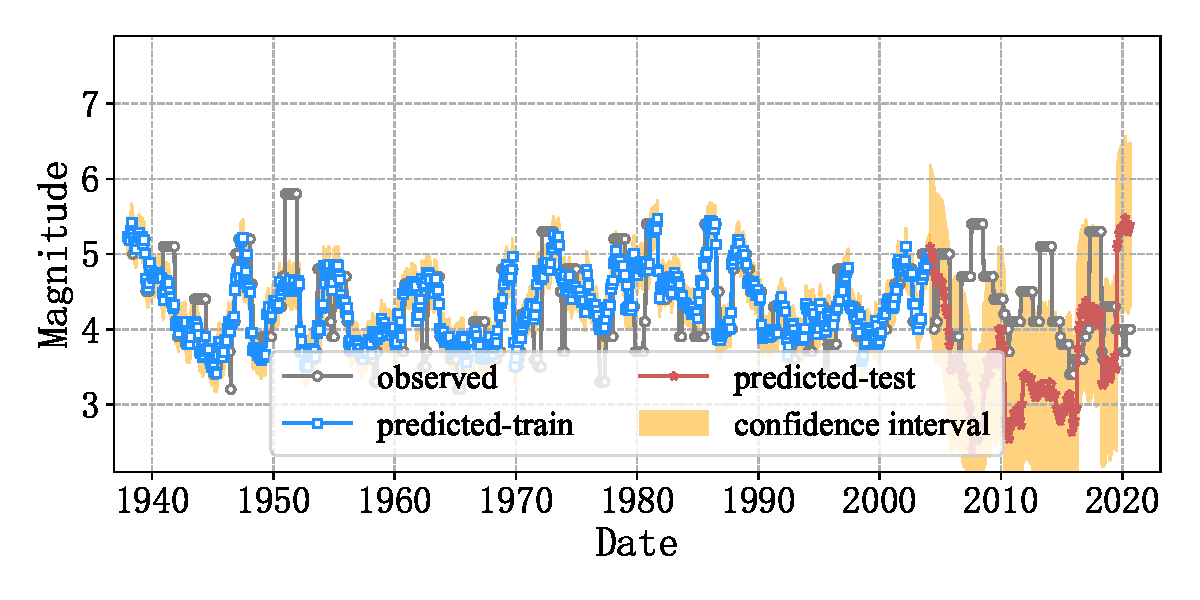
\includegraphics[width=\textwidth]{Img/chap5_seism/block6/seism_svr_minyear_1932_maxyear_2021_spanlat_2_spanlon_4_timewindow_72_nextmonth_12_minmag_3.0_block_6.pdf}
    \vspace{-1cm}
    \label{fig:seism_svr_minyear_1932_maxyear_2021_spanlat_2_spanlon_4_timewindow_72_nextmonth_12_minmag_3.0_block_6}
  \end{subfigure}   
  \\
  \begin{subfigure}[b]{0.45\textwidth}
    \caption{LR}
    \vspace{-0.2cm}
    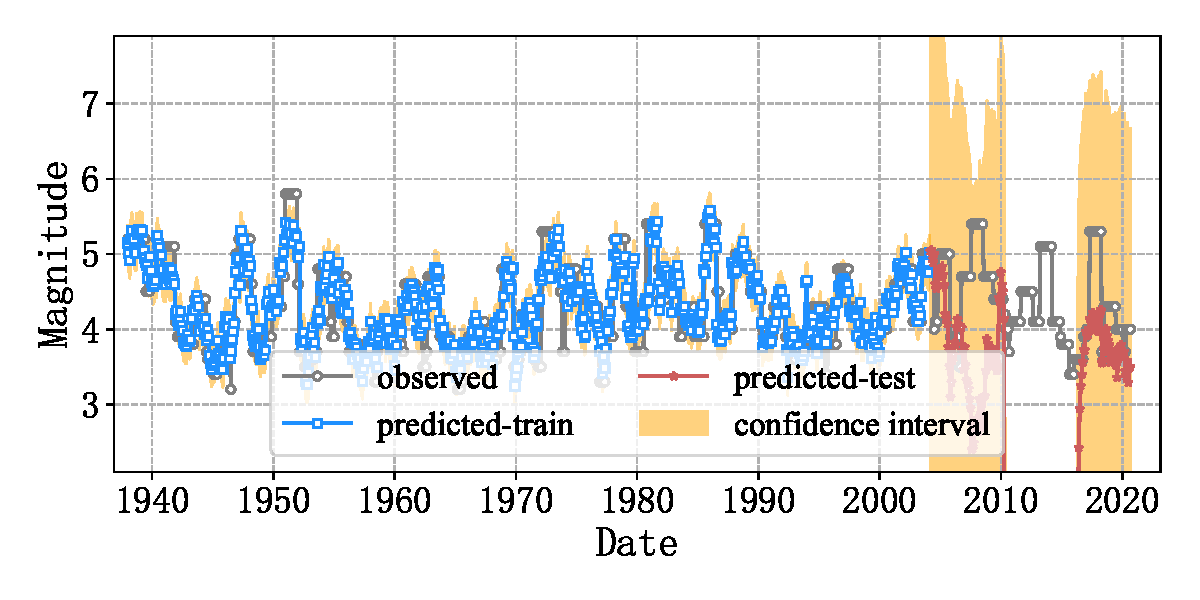
\includegraphics[width=\textwidth]{Img/chap5_seism/block6/seism_lr_minyear_1932_maxyear_2021_spanlat_2_spanlon_4_timewindow_72_nextmonth_12_minmag_3.0_block_6.pdf}
    \vspace{-1cm}
    \label{fig:seism_lr_minyear_1932_maxyear_2021_spanlat_2_spanlon_4_timewindow_72_nextmonth_12_minmag_3.0_block_6}
  \end{subfigure}
  ~
  \begin{subfigure}[b]{0.45\textwidth}
    \caption{RF}
    \vspace{-0.2cm}
    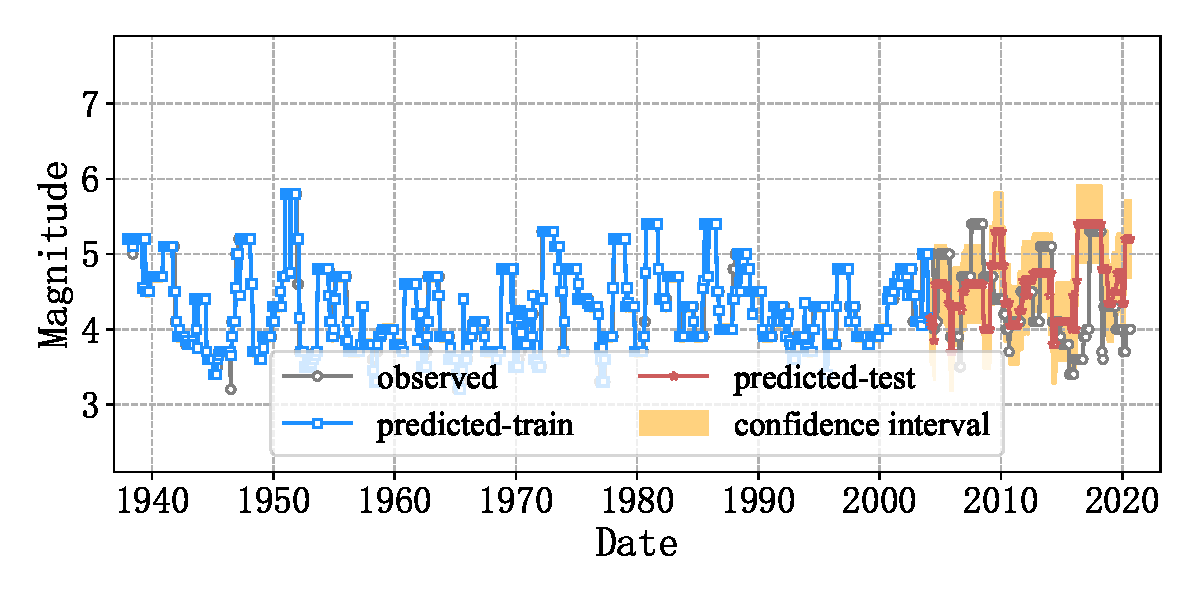
\includegraphics[width=\textwidth]{Img/chap5_seism/block6/seism_rf_minyear_1932_maxyear_2021_spanlat_2_spanlon_4_timewindow_72_nextmonth_12_minmag_3.0_block_6.pdf}
    \vspace{-1cm}
    \label{fig:seism_rf_minyear_1932_maxyear_2021_spanlat_2_spanlon_4_timewindow_72_nextmonth_12_minmag_3.0_block_6}
  \end{subfigure}
  \\
  \begin{subfigure}[b]{0.45\textwidth}
    \caption{GBRT}
    \vspace{-0.2cm}
    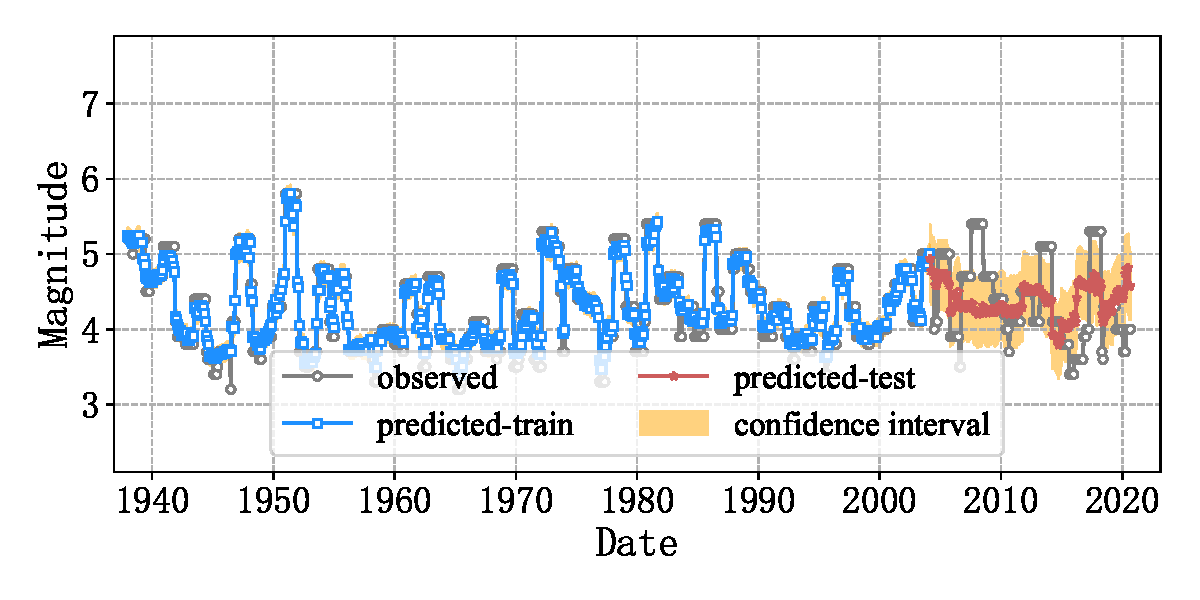
\includegraphics[width=\textwidth]{Img/chap5_seism/block6/seism_gbr_minyear_1932_maxyear_2021_spanlat_2_spanlon_4_timewindow_72_nextmonth_12_minmag_3.0_block_6.pdf}
    \vspace{-1cm}
    \label{fig:seism_gbr_minyear_1932_maxyear_2021_spanlat_2_spanlon_4_timewindow_72_nextmonth_12_minmag_3.0_block_6}
  \end{subfigure}
  ~
  \begin{subfigure}[b]{0.45\textwidth}
    \caption{DT}
    \vspace{-0.2cm}
    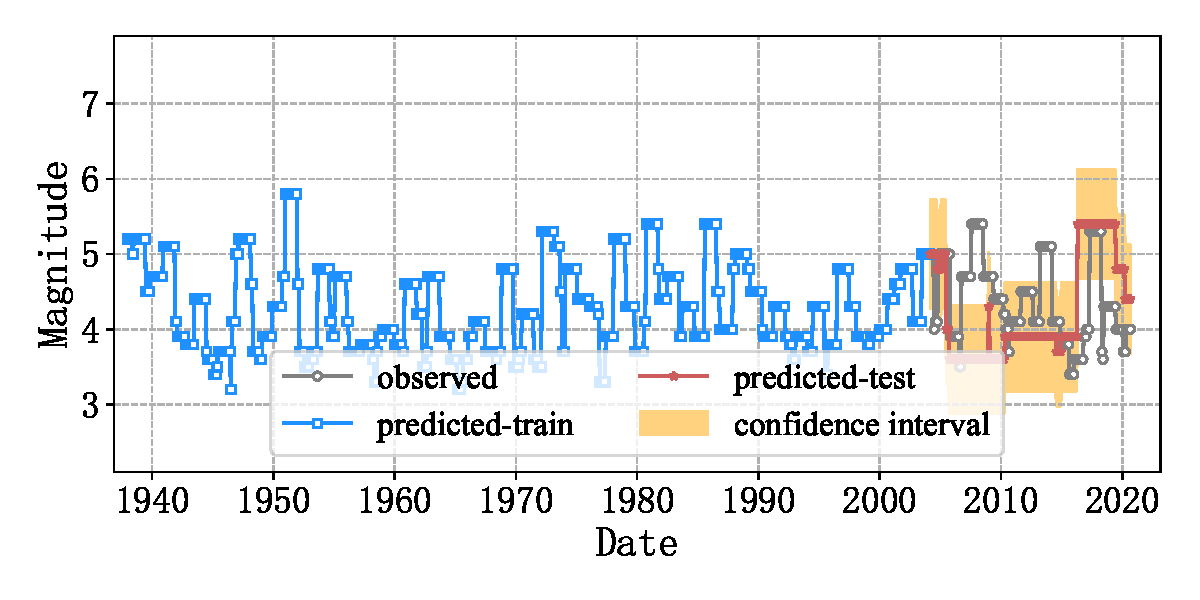
\includegraphics[width=\textwidth]{Img/chap5_seism/block6/seism_dt_minyear_1932_maxyear_2021_spanlat_2_spanlon_4_timewindow_72_nextmonth_12_minmag_3.0_block_6.pdf}
    \vspace{-1cm}
    \label{fig:seism_dt_minyear_1932_maxyear_2021_spanlat_2_spanlon_4_timewindow_72_nextmonth_12_minmag_3.0_block_6}
  \end{subfigure}
  \\
  \begin{subfigure}[b]{0.45\textwidth}
    \caption{KNN}
    \vspace{-0.2cm}
    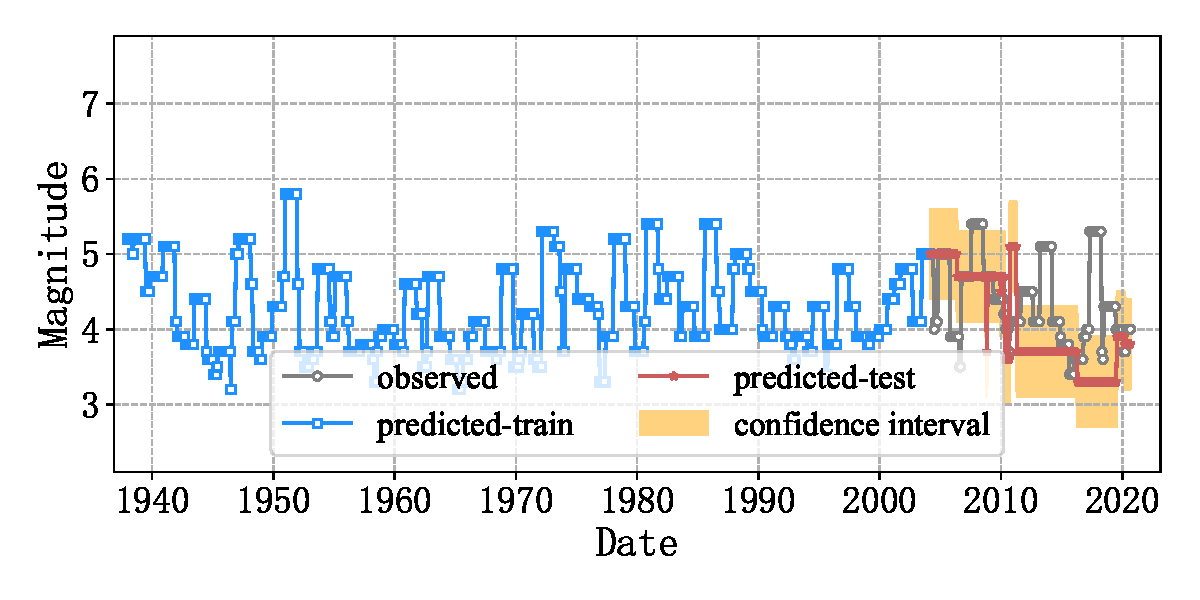
\includegraphics[width=\textwidth]{Img/chap5_seism/block6/seism_kn_minyear_1932_maxyear_2021_spanlat_2_spanlon_4_timewindow_72_nextmonth_12_minmag_3.0_block_6.pdf}
    \vspace{-1cm}
    \label{fig:seism_knn_minyear_1932_maxyear_2021_spanlat_2_spanlon_4_timewindow_72_nextmonth_12_minmag_3.0_block_6}
  \end{subfigure}
  ~
  \begin{subfigure}[b]{0.45\textwidth}
    \caption{ETR}
    \vspace{-0.2cm}
    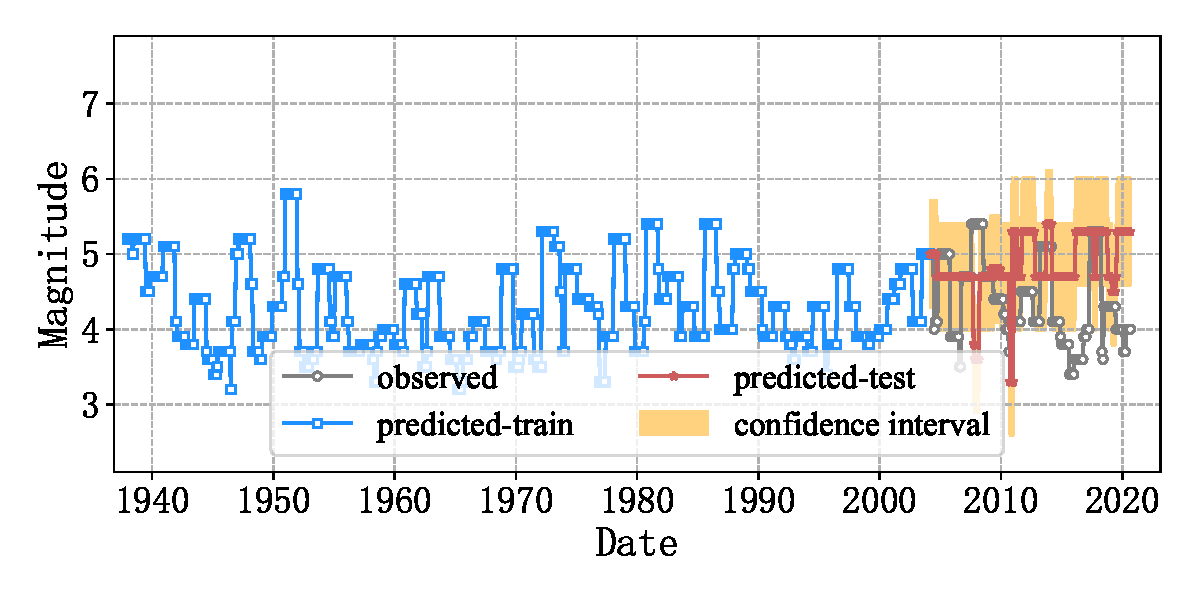
\includegraphics[width=\textwidth]{Img/chap5_seism/block6/seism_etr_minyear_1932_maxyear_2021_spanlat_2_spanlon_4_timewindow_72_nextmonth_12_minmag_3.0_block_6.pdf}
    \vspace{-1cm}
    \label{fig:seism_etr_minyear_1932_maxyear_2021_spanlat_2_spanlon_4_timewindow_72_nextmonth_12_minmag_3.0_block_6}
  \end{subfigure}
  \bicaption[不同模型预测区块6未来1年最大震级的时间序列图(数据集划分比例为0.8:0.2)]{不同模型预测区块6未来1年最大震级的时间序列图(数据集划分比例为0.8:0.2)。}{The time series of predicting the maximum magnitute of block 6 with the split ratio 0.8:0.2 in next year by different models.}
  \label{fig:seism_minyear_1932_maxyear_2021_spanlat_2_spanlon_4_timewindow_72_nextmonth_12_minmag_3.0_block_6}
\end{figure}